 \documentclass[
	11pt,
	openright,
	oneside,
	a4paper,
	english,
	french,
	spanish,
	brazil,	
	]{abntex2}

\usepackage{abntex2-cefetmg-timoteo}

\usepackage{cmap}
\usepackage{lmodern}
\usepackage[T1]{fontenc}
\usepackage[utf8]{inputenc}	
\usepackage{lastpage}
\usepackage{indentfirst}
\usepackage{color}
\usepackage{graphicx}
\PassOptionsToPackage{normalem}{ulem} 
\usepackage{ulem}
\usepackage{multicol}
\usepackage{multirow}
\usepackage{caption}
\usepackage{upgreek}
\usepackage{float}
\usepackage[most]{tcolorbox}
\usepackage{helvet}
\renewcommand{\familydefault}{\sfdefault}
\usepackage[brazilian,hyperpageref]{backref}
\usepackage[alf,abnt-thesis-year=both,]{abntex2cite}
\usepackage{longtable}
\usepackage{pdfpages}
\renewcommand{\backrefpagesname}{Citado na(s) página(s):~}
\renewcommand{\backref}{}
\renewcommand*{\backrefalt}[4]{
	\ifcase #1 
		Nenhuma citação no texto.
	\or
		Citado na página #2.
	\else
		Citado nas páginas #2.
	\fi}
\newcommand{\red}[1]{{\color{red}{#1}}}
\newcommand{\redb}[1]{{\color{red}\textbf{{#1}}}}
\newcommand{\quot}[1]{\begin{flushright} \textit{#1}\end{flushright}}


\titulo{Estudo de caso: utilização de redes adversárias geradoras para super-resolução de imagens científicas}
\autor{Leonam Teixeira de Vasconcelos}
\local{Timóteo}
\data{2025}
\orientador{Douglas Nunes de Oliveira}
\instituicao{
  Centro Federal de Educação Tecnológica de Minas Gerais
  \par
  Campus Timóteo
  \par
  Graduação em Engenharia de Computação
}
\tipotrabalho{Trabalho de conclusão de curso (Graduação)}
\preambulo{Monografia apresentada à Coordenação de Engenharia de Computação do Campus Timóteo do Centro Federal de Educação Tecnológica de Minas Gerais para obtenção do grau de Bacharel em Engenharia de Computação.}

\makeatletter
\hypersetup{
		pdftitle={\@title}, 
		pdfauthor={\@author},
    	pdfsubject={\imprimirpreambulo},
	    pdfcreator={LaTeX with abnTeX2},
		pdfkeywords={abnt}{latex}{abntex}{abntex2}{trabalho acadêmico}, 
		colorlinks=true,
    	linkcolor=black,
    	citecolor=black,
    	filecolor=black,
		urlcolor=black,
		bookmarksdepth=4
}
\makeatother


\setlength{\parindent}{1.3cm}

\setlength{\parskip}{0.2cm} 

\makeindex

\begin{document}

\frenchspacing 

 \pretextual

\imprimircapa

\imprimirfolhaderosto*

\includepdf[pages=-]{pdf_assets/folha_assinatura.pdf}

\begin{dedicatoria}
    \vspace*{\fill}
	\begin{flushright}
		Dedico aos meus pais, Léia e Manoel,\\ ao meu irmão, Luan \\ e à minha tia Néia.	
	\end{flushright}
\end{dedicatoria}

\begin{agradecimentos}

\quot{``O homem não é nada além daquilo\\que a educação faz dele.``\\Immanuel Kant}

A conclusão deste trabalho é um evento que, quando o comecei, aparentava estar muito distante no horizonte. Conciliar seu desenvolvimento com meu trabalho, e minha carreira em seus altos e baixos, foi uma tarefa árdua -- quase tão difícil quanto o desenvolvimento do trabalho em si. Mas aqui estou, redigindo a última seção do documento, algo que antes parecia tão longínquo.

Tal conclusão, deste trabalho e do curso, jamais seriam possíveis sem o fiel e consistente apoio de minha família, portanto devo sem mais delongas deixar meus mais sinceros agradecimentos à minha mãe Léia, meu pai Manoel e ao meu melhor amigo: meu irmão, Luan, que daqui a alguns anos, estará escrevendo um trabalho para este mesmo curso, nesta mesma instituição, neste mesmo molde. Não posso deixar de também agradecer, minha tia Néia, que sempre esteve ao meu lado e ao lado dos meus pais.

Seria injusto eu não dedicar, mesmo que brevemente os agradecimentos a todos os meus amigos, junto com os quais trilhei esse caminho e também sou grato a todo o apoio que me foi concedido pelos meus queridos amigos de trabalho, com quem passo a maior parte do meu tempo, mesmo que de forma virtual. Meus profundos agradecimentos, a todos meus amigos que acompanharam direta, ou indiretamente o esforço e dedicação por trás da conclusão deste curso.

E por último, nada mais justo que deixar meus agradecimentos aos professores e professoras que fizeram parte de minha educação e treinamento como engenheiro de computação. Alguns de seus ensinamentos, ainda uso diariamente no meu dia a dia.

\end{agradecimentos}

\setlength{\absparsep}{18pt} 
\begin{resumo}

\noindent 

O presente trabalho procura validar a viabilidade de treinamentos específicos sob algoritmos de aprendizado de máquina para aumentar a resolução de imagens. A área de inteligência artificial explorada são as redes adversárias geradoras (RAGs), uma tecnologia que durante o início da escrita deste trabalho, era relativamente nova no mercado. Para concentrar os esforços em um sub conjunto palpável de imagens, a super resolução é focada em bases de imagens médicas e astronômicas, ambas sendo obtidas de fontes públicas na internet. Apesar de facilmente encontradas, as imagens requerem tratamento para se adaptarem à estrutura dos modelos. Este tratamento também faz parte dos esforços deste trabalho. Um desafio inevitável e indispensável para alcançar os objetivos é a integração de diversos softwares de terceiros, necessários para que o treinamento das redes adversárias geradoras aconteça. O trabalho explora diversas fases contendo tarefas mecânicas, tornando automação uma alternativa pertinente. Os resultados do trabalho mostram que os benefícios de um treinamento especializado em um único tipo de imagens não são perceptíveis em relação a um treinamento feito a partir de uma base de imagens genérica, quando a infraestrutura utilizada para o treinamento é limitada. 

\noindent 
\textbf{Palavras-chave}: aprendizado de máquina, super resolução de imagens, redes adversárias geradoras.

\end{resumo}

\begin{resumo}[Abstract]
\begin{otherlanguage*}{english}

\noindent 

This work, seeks to validate the viability of specific training for machine learning algorithms, in order to increase images resolutions. The artificial intelligence branch explored in this work are the generative adversarial networks (GANs), a technology that, by the time of this writing, is relatively new to the industry. To concentrate the effort in a tangible image subset, the super resolution is focused in datasets containing medical and astronomical images, both being publicly available on the internet. Although the images can be easily found, they require extra treatment to adapt to the model's structures. This treatment is also accounted for in the efforts of this work. An inevitable and crucial challenge to reach the goals, is to integrate the myriad of third part softwares required for the machine learning training. This work explores several phases containing mechanical tasks, making automation a pertinent alternative. The results show that the benefits of a training with a specialized image base are not perceptible in comparison with a training done with a generic image base, when the infrastructure used for the training is limited.

\noindent  
\textbf{Keywords}: machine learning, image super resolution, generative adversarial networks.
\end{otherlanguage*}
\end{resumo}


\renewcommand*{\insertchapterspace}{} 

\pdfbookmark[0]{\listfigurename}{lof}
\listoffigures*
\cleardoublepage

\pdfbookmark[0]{\listtablename}{lot}
\listoftables*
\cleardoublepage

\begin{siglas}
    \item[BN]       \textit{Batch Normalization} (Normalização em lote, do inglês)
    \item[CNN]      \textit{Convolutional Neural Network} (Redes neurais convolucionais, do inglês)
    \item[CPU]      \textit{Central Processing Unit} (Unidade de processamento central, do inglês) 
    \item[CUDA]     \textit{Compute Unified Device Architecture} (Arquitetura de dispositivo de computação unificada, do inglês)
    \item[DICOM]    Sigla para \textit{Digital Imaging and Communications in Medicine}, um padrão de comunicação e gerenciamento de imagens para medicina
    \item[DVR]      \textit{Digital Video Recorder} (Gravadores de vídeo digital, do inglês)
    \item[ERGAS]    \textit{Erreur Relative Globale Adimensionnelle de Synthèse} (Erro adimensional de síntese global relativa, do francês)
    \item[ESRGAN]   \textit{Enhanced Super Resolution Generative Adversarial Networks} (Redes adversárias geradoras aprimoradas, para super resolução, do inglês)
    \item[ETE]      Erro do treinamento específico
    \item[ETG]      Erro do treinamento genérico
    \item[GAN]      \textit{Generative Adversarial Network} (Redes adversárias geradoras, do inglês)
    \item[GPU]      \textit{Graphics Processing Unit} (Unidade de processamento de gráficos, do inglês)
    \item[JPG]      Sigla para \textit{Joint Photographic Experts Group}, um formato de arquivos
    \item[JSON]     \textit{Javascript Object Notation} (Notação de objetos do Javascript, do inglês)
    \item[MLP]      \textit{Multilayer Perceptron} (Perceptron de múltiplas camadas, do inglês)
    \item[MRI]      \textit{Magnetic Resonance Imaging} (Imagem por ressonância magnética, do inglês)
    \item[MSE]      \textit{Mean Squared Error} (Erro quadrático médio, do inglês)
    \item[NBIA]     \textit{National Biomedic Imaging Archive} (Acervo nacional de imagens biomédicas, do inglês)
    \item[PNG]      Sigla para \textit{Portable Network Graphics}, um formato de arquivos
    \item[PSNR]     \textit{Peak Signal-to-Noise Ratio} (Relação sinal-ruído de pico, do inglês)
    \item[RAG]      Redes Adversárias Geradoras
    \item[RMSE]     \textit{Root Mean Squared Error} (Raiz do erro quadrático médio, do inglês)
    \item[SRGAN]    \textit{Super Resolution Generative Adversarial Networks} (Redes adversárias geradoras para super resolução, do inglês)
    \item[TE]       Treinamento Específico
    \item[TG]       Treinamento Genérico
    \item[TPU]      \textit{Tensor Processing Unit} (Unidade de processamento de tensores, do inglês)
\end{siglas}


\begin{simbolos}
    \item[$ \alpha $] Letra grega minúscula Alfa
    \item[$ \beta $] Letra grega maiúscula Beta
    \item[$ \gamma $] Letra grega minúscula Gama
    \item[$ \mu $]    Letra grega minúscula Mu ou Mi
    \item[$ \prod $]  Letra grega maiúscula Pi, símbolo matemático de produtório
    \item[$ \sigma $] Letra grega minúscula Sigma
    \item[$ \sum $]   Letra grega maiúscula Sigma, símbolo matemático de somatório
    \item[$ \omega $] Letra grega minúscula Ômega
    \item[$ \infty $] Símbolo matemático para infinito
\end{simbolos}


\include{src/inicio/sumario}

\textual

\chapter[Introdução]{Introdução}
\quot{``As coisas nas quais você pensa\\determinam a qualidade da tua mente.''\\Marco Aurélio}
\label{chapter:introducao}
Na era da informação, uma quantidade avassaladora de dados sem precedentes é trafegada de dispositivo a dispositivo a cada segundo. Consumimos e produzimos um volume muito grande de informação. Em média o ser humano produziu cerca de 1,7MB de dados por minuto em 2020 \cite{vish_how_2020} e esse número só tende a aumentar. Uma parte significativa do conteúdo produzido e consumido é em forma de imagens (fotos e vídeos, se pensarmos que os vídeos são apenas imagens sendo reproduzidas em determinada frequência). Se avaliarmos que a cada iteração tecnológica, celulares e câmeras ficam melhores, capturando imagens maiores, com mais qualidade, resolução, alcance dinâmico etc. a variação da quantidade de dados produzidos está em ascensão.

Outro tipo de imagem pouco utilizada pelo público geral e de grande importância para o público científico são imagens de registros históricos, astronômicas e médicos. A razão pela qual estes três gêneros de imagens foram listados em conjunto é simples. Existe um conjunto grande dessas imagens em acervos de fotografia que possuem baixa qualidade, seja pela tecnologia obsoleta utilizada na época ou pela complexidade e custos para capturar uma imagem de mais qualidade. Algumas imagens médicas em particular como Ressonância Magnética, não podem, em alguns casos ser obtidas com uma qualidade maior devido à consequências à saúde do paciente exposto ao equipamento \cite{gupta_super-resolution_2020}.

\section{Justificativa}
\label{justificativa}

Para ambos os casos citados (número de imagens e vídeos crescendo com o avanço tecnológico e imagens científicas de baixa qualidade) poderíamos utilizar alguma forma de descompressão para aliviar as consequências do aumento absurdo da quantidade de imagens criadas e consumidas e da baixa qualidade das imagens históricas, médicas e astronômicas \cite{sun_super_2019,noauthor_review_2020}. No primeiro caso, poderíamos reduzir a resolução das imagens propositalmente para que essas ocupem menos espaço de armazenamento nos dispositivos e menos banda durante as transferências, aumentando inclusive, a velocidade destas. Para visualizar a imagem em uma qualidade mais alta (tanto as imagens propositalmente reduzidas quanto as imagens já com qualidade baixa) se faz necessário então uma forma viável de aumentar a resolução dessas imagens. 

O processo de aumentar a resolução de uma imagem é cientificamente conhecido como Super-resolução ou SISR (Single Image Super Resolution, Super-resolução de imagem única, do inglês) e é conhecido como um problema altamente dependente dos dados de entrada e que possui múltiplas soluções visto que para uma imagem de baixa resolução existem várias imagens que podem tê-la gerado  \cite{zhu_gan-based_2020}. Métodos algorítmicos baseados em conceitos matemáticos e sistemas baseados em aprendizado de máquina já existem para esse tipo de tarefa \cite{takemura_algoritmos_nodate, khaledyan_low-cost_2020}. No entanto, recuperar detalhes finos, como texturas, ao aumentar a resolução de imagens em um fator alto. ainda é um problema remanescente \cite{ledig_photo-realistic_2017}.

Uma técnica relativamente nova introduzida em 2016 por \citeonline{goodfellow_generative_2014, goodfellow_nips_2017}, faz o uso de várias redes neurais, competindo entre si para que em vez de manipularmos uma entrada e obter um resultado, possamos gerar um resultado novo a partir de aprendizado prévio. Essas redes são chamadas de Redes Geradoras Adversárias e foram desenvolvidas para que possamos gerar bases de dados novas e inéditas a partir de dados existentes \cite{goodfellow_generative_2014, moreira_geracao_2019} e já foram utilizadas para super-resolução de imagens, como mostra \citeonline{moreira_geracao_2019}. O trabalho, no entanto, deixa em aberto algumas propostas futuras para que possamos investigar novas formas de avaliar o desempenho deste método, assim como sugestões de novas formas com as quais podemos o mensurar e julgar. Seria possível combinar estes trabalhos com o propósito de desenvolver um modelo viável para esse tipo de problema? 

Este é o objetivo deste trabalho. Utilizar redes geradoras adversárias, reproduzindo e experimentando os trabalhos de \citeonline{ledig_photo-realistic_2017} e \citeonline{wang_esrgan_2018}, tendo como base de conhecimento a grande contribuição de \citeonline{goodfellow_generative_2014} para a ciência da computação e o trabalho de \citeonline{moreira_geracao_2019} a fim de treinar um modelo onde possamos recuperar qualidade de uma imagem de baixa qualidade. Para seguir a linha de pesquisa dos autores mencionados, o trabalho foca em super-resolução de imagens científicas, mais especificamente, imagens astronômicas e médicas de aparelhos utilizados para exames de imagem, como ressonância magnética. 

Dessa forma, é possível verificar o desempenho dessa metodologia no âmbito científico, recuperando ou aprimorando fotos precárias, ou de qualidade indesejável (como mencionado em \citeonline{sun_super_2019, noauthor_review_2020, gupta_super-resolution_2020}). 

\section{Objetivos}

Experimentar os trabalhos de \citeonline{ledig_photo-realistic_2017, moreira_geracao_2019, wang_esrgan_2018} para a elaboração de uma rede geradora adversária treinada especificamente para a super-resolução de imagens científicas a fim de validarmos os custos e benefícios deste treinamento específico em relação à modelos genericamente treinados.

Mais especificamente, os objetivos do trabalho podem ser sumarizados nos tópicos abaixo:

\begin{enumerate}

    \item Definir um sub-conjunto de imagens, especificamente de uma ou duas áreas para especializarmos o modelo

    \item Definir um modelo de redes geradoras adversárias para o contexto apresentado
	
    \item Integrar todo software e dependência necessários para treinar e utilizar o modelo escolhido no objetivo anterior
    
	\item Definir as bases de imagens para treinar o modelo escolhido de forma específica
	
	\item Utilizar-se de técnicas de cálculo de similaridade de imagens para avaliar o desempenho do treinamento realizado

\end{enumerate}
 


\chapter{Revisão bibliográfica}
\quot{``Ler, é pensar com uma cabeça alheia''.\\Arthur Schopenhauer}
\label{chapter:metodologia}
\label{metodologia}

\section{Trabalhos correlatos}

As principais fontes para este trabalho se concentram principalmente em livros e artigos recentes, assim como artigos de sites online em alguns pontos específicos. Serão utilizados também alguns materiais mais antigos, especialmente na parte onde estarei fundamentando o conhecimento base (neurônios artificiais, redes neurais etc.). Estes trabalhos e técnicas já estão estabelecidos no meio acadêmico e suas citações são necessárias. Os artigos científicos foram obtidos de três fontes principais: Google Acadêmico, Portal de Periódico CAPES e \textit{Arxiv}.

Ledig, et al. \cite{ledig_photo-realistic_2017} desenvolveram uma arquitetura de redes geradoras adversárias (\ref{sec:gan}) que possui desempenho superior à outras técnicas no âmbito de super-resolução de imagens. O trabalho publicado, está gratuitamente disponível no repositório \textit{Arxiv} e será de suma importância para este trabalho. Pode-se dizer que este artigo foi a principal inspiração para o tema. Posteriormente, em 2018, \cite{wang_esrgan_2018} resolveu otimizar o modelo gerador proposto por \cite{ledig_photo-realistic_2016}. O autor identificou que para a forma com a qual o artigo inicial calcula os erros da rede geradora, a arquitetura não está otimizada. Foi proposta e implementada então, uma otimização para o modelo, que traz melhor desempenho no treinamento e resultados mais satisfatórios.



\section{Super resolução de imagens}
\label{sec:sisr}

Super-resolução de imagens, é o processo de, artificialmente, produzir uma imagem de alta resolução a partir de uma imagem de baixa resolução. De acordo com \citeonline{nasrollahi_super-resolution_2014}, o objetivo da super-resolução de imagens, é aumentar a quantidade de \textit{pixels} por unidade de área em uma imagem, aumentando assim o nível de detalhes se compararmos o resultado, com a imagem original. Ainda de acordo com os autores citados anteriormente, inúmeras aplicações de super-resolução de imagens foram e são exploradas, e diversas técnicas para se performar a super-resolução de imagens são conhecidas hoje em dia. A figura \ref{fig:super-resolucao:fig11} abaixo, mostra as diferentes abordagens disponíveis para realizar super-resolução de imagens. 

\begin{figure}
    \centering
    \caption{Diagrama de diferentes áreas da super-resolução de imagens.}
    \includegraphics[width=11cm]{fig/SR-Taxidermy.png}
    \legend{Fonte: \cite{nasrollahi_super-resolution_2014}}
    \label{fig:super-resolucao:fig11}
\end{figure}

Como a imagem \ref{fig:super-resolucao:fig11} indica, a super-resolução de imagens, pode ser realizada utilizando diversos artifícios e algoritmos diferentes. Algumas das estratégias utilizadas para tal são rápidas e computacionalmente simples, como filtragem linear, bicúbica e Lanczos, porém produzem resultados de baixa qualidade \cite{ledig_photo-realistic_2016}. Estes métodos simplificam demasiadamente o problema de ampliar a resolução de uma imagem. Métodos envolvendo redes neurais convolucionais têm mostrado grande desempenho para a tarefa de aumentar a resolução de imagens \cite{ledig_photo-realistic_2016, dong_image_2015}. Estes métodos aprendem padrões espaciais das imagens de entrada, sendo capazes de extrair detalhes e características da imagem e aplicar nesta, o modelo. A figura \ref{fig:super-resolucao:fig14}, traz três exemplos de super-resolução: interpolação bicúbica, rede profunda residual e redes adversárias generativas, da esquerda para direita. Na extrema direita, está a imagem original, para fins de comparação.

\begin{figure}[H]
    \centering
    \caption{Diferentes métodos para super-resolução de imagens.}
    \includegraphics[width=12cm]{fig/SISR.png}
    \legend{Fonte: \cite{ledig_photo-realistic_2016}}
    \label{fig:super-resolucao:fig14}
\end{figure}


\section{Redes neurais artificiais}
\label{sec:rna}
\index{MLP}
\index{RNA}
\index{Redes Neurais Artificiais}

Este trabalho é fortemente apoiado em redes neurais. Toda a fundamentação posterior possui-as como base para algo um pouco mais complexo. Portanto, um conhecimento sólido deste tópico, é um requisito indispensável. Redes neurais, de acordo com \cite{haykin_redes_2007}, são definidas como "[...] um processador maciçamente paralelamente distribuído constituído de unidades de processamento simples, que têm a propensão natural para armazenar conhecimento experimental e torná-lo disponível para uso." (HAYKIN, 2007, p.28). De forma simplória, uma rede neural consiste em componentes simples, que apesar de isolados não serem capazes de generalizar ou aprender complexidade exorbitante, quando organizados em conjuntos estruturados, contribuem individualmente para que a rede como um todo seja capaz de realizar tarefas mais complicadas.

Estas unidades simples de processamentos são conhecidas como \textit{neurônios artificiais} e a rede neural, é um conjunto destes neurônios interligados de uma maneira específica. Um neurônio pode ser definido como uma estrutura que possui três características básicas: um conjunto de conexões (conhecidas tecnicamente como \textit{sinapses}), uma forma de combinar sinais de entrada e uma função de ativação \cite{haykin_redes_2007}. 

As sinapses representam as conexões feitas entre neurônios e compreendem sinais de entradas sendo calibrados pelo peso da conexão. No modelo mais simples de redes neurais, esta calibração é feita em forma de multiplicação, ou seja, um sinal de entrada $x_i$ é multiplicado pelo peso sináptico $w_i$ para obtermos a sinapse $i$. Como dito anteriormente, um neurônio possui um conjunto de sinapses e os valores computados por estas precisam ser combinados de alguma forma. Uma das formas de calcular tal combinação é fazendo o simples somatório do valor das sinapses, obtendo assim uma saída para aquele neurônio. 

A função de ativação modula esta saída de acordo com a necessidade. Talvez o problema a ser resolvido requeira limitar a saída deste neurônio para um intervalo arbitrário, ou talvez converter a saída em um conjunto limitado de valores. A função de ativação é a responsável por esta tarefa. A figura \ref{fig:fig1}, descreve visualmente como um neurônio artificial é representado matemática e computacionalmente. Na imagem, os \textit{inputs} são os sinais de entrada; \textit{weights} são os pesos sinápticos; \textit{transfer function} é o combinador interno (o símbolo grego $\Sigma$ [sigma] indica um somatório); e \textit{activation function}, representada por $\upvarphi$ é a função de ativação. Para implementar esta arquitetura programaticamente, utiliza-se de operações matriciais para calcular a saída do neurônio, em relação às suas entradas ponderadas por seus respectivos pesos.

\begin{figure}[H]
    \centering
    \caption{Diagrama de um neurônio artificial.}
    \includegraphics[width=8cm]{fig/ArtificialNeuronModel.png}
    \legend{Fonte: \cite{chrislb_english_2005}}
    \label{fig:fig1}
\end{figure}

Inspirado pela forma como nosso cérebro funciona e computa, o neurônio artificial foi primeiramente desenvolvido em 1943 por McCulloch e Pitts e ficou conhecido como \textit{modelo de McCulloch-Pitts} \cite{mcculloch_logical_1943}. Apesar de inovador, o neurônio tem suas limitações. Um único neurônio está limitado a problemas linearmente separáveis \cite{haykin_redes_2007}. Esta limitação trouxe uma estagnação na área de inteligência artificial em torno do neurônio por alguns anos. 

Posteriormente, o neurônio foi organizado em camadas, formando assim, uma rede neural onde agora, os problemas aplicáveis não precisam ser necessariamente linearmente separáveis. A imagem \ref{fig:fig2} mostra como tal estrutura de neurônios é organizada, onde \textit{hidden layer} é uma camada intermediária, ou uma camada escondida e \textit{output layer} é a camada de saída. Cada círculo representa um neurônio e as setas, a ligação entre estes.

\begin{figure}[H]
    \centering
    \caption{Diagrama de uma rede neural ou de um perceptron de múltiplas camadas.}
    \includegraphics[width=8cm]{fig/MultiLayerNeuralNetwork_english.png}
    \legend{Fonte: \cite{wikimedia_multilayerneuralnetwork_2021}}
    \label{fig:fig2}
\end{figure}

\index{MLP} \index{Multilayer Perceptron}

O sinal de entrada desta rede, é propagado da entrada para a saída, em forma de uma série de operações matemáticas. O princípio de funcionamento do neurônio continua o mesmo: os sinais de entrada são balanceados pelo peso das ligações, combinados internamente e calibrados pela função de ativação. Agora no entanto, a saída deste neurônio é propagada para todo neurônio que recebe seu sinal de saída como entrada. Vide figura \ref{fig:fig3}. A saída do neurônio \textit{A} é propagada para todos os neurônios que possuem-a como entrada: neurônios \textit{B} e \textit{C}.

\begin{figure}[H]
    \centering
    \caption{Diagrama de uma rede neural ou de um perceptron de múltiplas camadas com fluxo de dados. }
    \includegraphics[width=8cm]{fig/MLP.png}
    \legend{Fonte: autor}
    \label{fig:fig3}
\end{figure}

Estas redes foram e são amplamente utilizadas para os mais diversos tipos de classificação e modelagem de dados, porém, por maior que seja sua capacidade de generalização e aprendizado, este modelo em específico é insuficiente para se capturar padrões espaciais em determinados tipos de dados. Isto é, é possível encontrar padrões entre números mas estes modelos não dependem da ordem da entrada. Caso a entrada seja uma imagem, em um perceptron de múltiplas camadas (considere uma imagem preto e branca representada como uma matriz de \textit{NxM} onde cada posição corresponde ao valor do pixel da imagem naquele local), não faz diferença se a imagem em forma de matriz for remodelada em um vetor, retirando assim uma dimensão da estrutura \cite{zhang_dive_2021}. De forma mais simples, este modelo tem dificuldades em aprender padrões que representam o relacionamento de um dado com seus adjacentes, como um pixel e a forma como este interfere com os pixels ao seu redor e por estes é afetado.


\section{Redes neurais convolucionais}
\label{sec:cnn}
\index{Redes neurais convolucionais}
\index{CNN}
\index{RNC}

Redes neurais convolucionais foram desenvolvidas para resolver o problema de aprender o relacionamento entre dados adjacentes e são amplamente utilizadas para o processamento de imagens justamente por terem a capacidade de extrair características úteis para reconhecimento de objetos e classificação. Este modelo possui inspiração na biologia, teoria de grupos entre outros \cite{zhang_dive_2021}. Nesta seção as redes neurais convolucionais serão introduzidas.

Convolução é um conceito matemático que é calculado entre duas funções \textit{f} e \textit{g} e mede o quanto a função \textit{g} se sobrepõe à função \textit{f} se \textit{g} se desloca através de \textit{f} e é calculada formalmente como \cite{wikipedia_convolucao_2020, weisstein_convolution_2003, zhang_dive_2021}:

\begin{equation}
    (f * g)(x) = \int f(z)g(x-z)dz
    \label{eq:eq1}
\end{equation}

A equação \ref{eq:eq1} pode ser generalizada para múltiplas dimensões, como é o caso de imagens. Imagens em preto e branco podem ser definidas com duas dimensões (largura e altura) enquanto imagens coloridas podem ser definidas com três dimensões (largura, altura e cor). 

Para detectar um objeto em específico em uma imagem, considerando que o modelo matemático desta esteja disponível, pode-se calcular a convolução da primeira imagem em relação ao objeto. Assim, os pontos mais propensos de se encontrar o objeto terão um pico na convolução \cite{zhang_dive_2021}. No caso de imagens coloridas, essas convoluções devem ser adaptadas para trabalhar com canais de cores diferentes (vermelho, verde e azul): os três canais que compõem uma imagem colorida. As convoluções extraem características da imagem e reduzem a complexidade do processamento. De acordo com \citeonline{zhang_dive_2021}, camadas de convoluções geralmente requerem menos parâmetros que uma rede completamente conectada, como um MLP. \index{MLP} \index{Multilayer Perceptron}

Para capturar detalhes espaciais de uma imagem, as redes convolucionais conectam um conjunto de pixels adjacentes em um único neurônio da próxima camada. Este neurônio tem um nome especial. É conhecido como \textit{campo receptivo local}. Esta operação que acaba de ser descrita é uma convolução \cite{gulli_deep_2019}. Veja a imagem abaixo:

\begin{figure}[H]
    \centering
    \caption{Exemplo de operação de convolução. Os números foram propositalmente colocados de forma repetitiva para facilitar a explicação e os cálculos.}
    \includegraphics[width=12cm]{fig/conv.png}
    \legend{Fonte: autor, baseado em \cite{zhang_dive_2021}}
    \label{fig:fig4}
\end{figure}

Na figura \ref{fig:fig4}, a matriz de entrada representa uma imagem e a matriz \textit{K} é a matriz com a qual iremos fazer a convolução da imagem. Em redes convolucionais (chamaremos de CNN a partir de agora para sermos mais breve. CNN vem do inglês, \textit{convolutional neural networks} que traduz diretamente para redes neurais convolucionais), essa matriz \textit{K} é chamada de \textit{kernel} ou \textit{núcleo}, em português. Esta matriz é responsável por extrair informações da imagem. No exemplo anterior, da figura \ref{fig:fig4}, durante cada iteração da convolução, sobrepõe-se um subconjunto de pixels da imagem. Na primeira iteração, ela sobrepõe os pixels pintados em amarelo e o resultado desta convolução é 10 (2*1 + 2*0 + 2*1 + 2*0 + 2*1 + 2*0 + 2*1 + 2*0 + 2*1 = 10), portanto, na próxima camada, temos uma saída no valor de 10. Na próxima iteração, a matriz núcleo se desloca em um pixel para a direita e faz a mesma operação. Quando ela atinge o final da matriz de imagem, volta ao início e desloca um pixel abaixo, e assim por diante até cobrir toda a imagem. Por meio dessas operações, somos capazes de aproveitar e aprender o relacionamento entre pixels adjacentes, algo que não é tão simples de se fazer com uma rede MLP.

Além de convoluções, uma funcionalidade importante em redes convolucionais, é o \textit{pooling}. Esta operação reduz a complexidade e a resolução das características agregadas e aprendendidas de uma imagem a medida que o processamento da imagem acontece. No final das contas, o objetivo é capturar detalhes específicos da imagem. Estes detalhes, devem ser suficientes para se extrair a informação necessária. Identificar um objeto em uma imagem como um cachorro, uma pessoa, um carro etc. por exemplo. As ultimas camadas da rede devem ser bastante sensíveis à imagem de entrada, de forma que se a alterarmos minimamente, a alteração trará consequências significativas ao resultado final. A saída de uma camada de convolução é chamada de \textit{feature map} (mapa de atributos, do inglês) \cite{zhang_dive_2021, brownlee_gentle_nodate}. 

Existem várias formas de se fazer o \textit{pooling}, entre elas temos \textit{max pooling} e \textit{average pooling}.

\subsection{Max Pooling}

Para fazer o \textit{max pooling} de uma matriz, seleciona-se um subconjunto de seus pixels, representando-os como um único dado para a próxima camada: o pixel com o maior valor \cite{zhang_dive_2021, brownlee_gentle_nodate}. O diagrama abaixo (figura \ref{fig:fig5} ilustra de forma simplória a técnica de \textit{max pooling}. Da esquerda para direita, e cima para baixo a operação opera sobre toda a matriz. Percebe-se que alguns valores aprecem mais vezes. Talvez reduzir o tamanho da matriz de \textit{pooling} (conhecida também como janela de \textit{pooling}) ou normalizar os \textit{pixels} da imagem antes do processamento, seja uma forma de evitar tais repetições excessivas.

\begin{figure}[H]
    \centering
    \caption{Exemplo de operação de \textit{max pooling}.}
    \includegraphics[width=13cm]{fig/Max Pooling.png}
    \legend{Fonte: autor, baseado em \cite{zhang_dive_2021, gulli_deep_2019}}
    \label{fig:fig5}
\end{figure}

\subsection{Average Pooling}

Esta operação é bastante parecida com o \textit{max pooling} na forma como é realizada, porém o cálculo é diferente. Em vez de se calcular o valor máximo dos pixels da matriz de entrada, calcula-se a média aritmética \cite{zhang_dive_2021, brownlee_gentle_nodate}. O diagrama abaixo ilustra o que foi dito:

\begin{figure}[H]
    \centering
    \caption{Exemplo de operação de \textit{average pooling}. Da esquerda para direita, e cima para baixo a operação é realizada sobre toda a matriz.}
    \includegraphics[width=13cm]{fig/Avg Pooling.png}
    \legend{Fonte: autor, baseado em \cite{zhang_dive_2021, gulli_deep_2019}.}
    \label{fig:fig6}
\end{figure}

\subsection{A arquitetura da rede}

Redes convolucionais podem ser organizadas das mais variadas maneiras existentes para as mais variadas tarefas. Duas formas famosas na literatura, são as redes convolucionais para classificação que terminam completamente conectadas e as completamente convolucionais. A primeira arquitetura consiste em uma CNN tradicional, com as camadas de convolução e \textit{pooling}, porém no final ela se conecta a uma rede completamente conectada (i.e. cada neurônio da camada anterior se conecta a todos neurônios da próxima camada) como um MLP e a partir dele pode classificar o conteúdo de uma imagem, como o exemplo famoso de detectar se o objeto da foto é um cachorro ou um gato. Nesse caso, a CNN irá extrair das imagens as características necessárias para avaliar o que o objeto é. Com as características extraídas, estas são alimentadas na rede completamente conectada e esta por sua vez faz a classificação.

A segunda arquitetura não envolve camadas completamente conectadas. Neste modelo, a rede mantém a estrutura da CNN até a última camada. Um exemplo de aplicação desta arquitetura, é a segmentação de imagens. Aproveitando o caso de uso da arquitetura anterior, suponha que em vez de identificar se na imagem há um gato ou um cachorro, o objetivo seja descobrir onde especificamente, naquela imagem está o cachorro. Para esta funcionalidade, a rede precisaria de não apenas detectar as características da imagem e identificar o cachorro, como também precisaria demarcar o animal na imagem. Para isso, essas redes utilizam as características extraídas nas camadas iniciais para reconstruir a imagem nas camadas finais, destacando o objeto em questão \cite{kumar_semantic_2020}.

Para este trabalho, ambas as arquiteturas serão utilizadas. Nas próximas seções, ficará mais claro a aplicação de cada uma destas.


\section{Treinamento da rede}
\label{sec:train}
\index{Treinamento da rede} 
\index{Backpropagation}

Para que redes neurais aprendam, estas precisam ser submetidas a um processo de treinamento, que no caso de redes neurais, representa uma técnica de ajuste dos pesos sinápticos, a fim de reduzirmos o erro da rede. Existem várias formas de treinar uma rede neural, e uma das mais famosas é a retro propagação do erro, conhecida popularmente pelo termo em inglês \textit{backpropagation} \cite{rumelhart_learning_1986}. Como o nome sugere, o treinamento é realizado perante à disseminação do erro obtido pela rede, de trás pra frente. Isto é, para ajustar os pesos da rede utilizando este algoritmo, insere-se na rede uma entrada da qual a saída esperada é conhecida. Calcula-se então, a diferença entre a saída esperada e obtida. Os pesos em seguida, sãp atualizados proporcionalmente a este erro, levando também em consideração o quanto cada peso interfere no erro, da camada mais profunda, para a camada menos profunda \cite{rumelhart_learning_1986}. A fim de se otimizar este treinamento, existem ferramentas matemáticas para atualizarmos os pesos de formas mais eficientes.

Em 1944, um matemático chamado Haskell B. Curry, descreveu a aplicação de um método já conhecido para a otimização de problemas, que posteriormente ficou conhecido como \textit{Gradient Descent} \cite{curry_method_1944}. Este método utiliza um conceito matemático chamado gradiente, para encontrar a direção mais eficiente para o mínimo de uma função. O gradiente é um vetor de \textit{n} componentes, onde \textit{n} é a dimensão da função a ser otimizada, que no caso do treinamento, é a função que representa o erro da rede neural, em função de todos seus parâmetros treináveis, como seus pesos. Quando o gradiente desta função é calculado, sabe-se, exatamente em qual direção os erros devem ser atualizado para se alcançar o mínimo, o mais rápido possível (com o menor número de iterações de treinamento), diminuindo assim, a complexidade e o tempo necessários para o treinamento.

Retro-propagação do erro em conjunto com o \textit{Gradient Descent} compõem o algoritmo ótimo de treinamento. Com a retro-propagação, altera-se o peso individual, proporcionalmente ao quanto este, interfere no erro. O gradiente então, fornece o caminho mais rápido para minimizar este erro. Para que estas operações sejam realizadas, uma série de cálculos matemáticos são realizadas a cada etapa de treinamento, fazendo com que a a complexidade desta fase crucial no desenvolvimento de redes neurais seja uma das mais demoradas e computacionalmente exaustivas.

Apesar de o tópico de treinamento de redes neurais ser de suma importância nos estudos de inteligência artificial, é externo ao objetivo deste trabalho, descrever em fino detalhe tal atividade. As bibliotecas de inteligência artificial amplamente utilizadas na indústria, que serão utilizadas na parte prática do presente trabalho, abstraem grande parte da complexidade matemática e algebraica do treinamento. Portanto, maiores detalhes sobre treinamento de redes neurais serão omitidos.


\section{Redes Adversárias Geradoras}
\label{sec:gan}
\index{GAN}
\index{RAG}
\index{Redes Adversárias Geradoras}

Uma forma relativamente nova na indústria para gerar dados, é a utilização das \textit{redes geradoras adversárias}\index{GAN}. O conceito foi introduzido em 2014 por Ian Goodfellow \cite{goodfellow_generative_2014}. As redes geradoras utilizam o princípio da competição para produzir os resultados e para disso, utiliza (pelo menos na arquitetura inicial proposta) duas redes neurais, competindo entre si para gerar quaisquer forma de dados que sejam aplicáveis à esse tipo de modelo.

O modelo consiste de duas redes neurais denominadas \textit{geradora} ($G(x)$) e \textit{discriminadora} ($D(y)$). A geradora, como o próprio nome diz gera o dado em questão: imagens, texto, música entre outros \cite{c_han_gan-based_2018, xu_diversity-promoting_2018, oza_progressive_2019}. 

A rede discriminadora, tem uma função simples: validar o que a geradora produz. Esta rede detecta se o que foi produzido pela geradora é falso ou não. Seja o problema de se implementar uma RAG (sigla para redes geradoras adversárias) capaz de gerar imagens de pôr do sol. A rede discriminadora será treinada para identificar o que é e o que não é uma imagem de pôr do sol enquanto a rede geradora será treinada para a enganar. Taí a competição: enquanto a rede \textit{D} fica melhor em detectar se uma imagem é falsa ou não, a rede \textit{G} fica melhor em enganar a rede \textit{D} a achar se que o que ela está produzindo, é uma imagem verdadeira de pôr do sol.

\begin{figure}[H]
    \centering
    \caption{Diagrama de uma RAG.}
    \includegraphics[width=11cm]{fig/GAN_2.png}
    \legend{Fonte: autor, baseado em \cite{gulli_deep_2019, zhang_dive_2021, moreira_geracao_2019}.}
    \label{fig:fig7}
\end{figure}

De acordo com a imagem \ref{fig:fig7}, a saída da rede geradora alimenta a rede discriminadora, assim como dados reais também entram nesta. Estes são utilizados para treiná-la a diferenciar com cada vez mais precisão um dado falso de um verdadeiro (ou, gerado de real). No caso de super-resolução de imagens, estes dados são em forma de imagens. A geradora é treinada para converter ruído em imagens. Imagens estas, que por sua vez sejam capazes de enganar a discriminadora a classificar se a imagem gerada é uma imagem verdadeira. Uma vez que as imagens artificialmente geradas são capazes de se passarem por imagens verdadeiras (entenda \textit{se passarem por imagens verdadeiras} como serem identificadas como imagens reais), a rede geradora estará produzindo imagens semelhantes às imagens nas quais a rede discriminadora foi treinada para identificar. O termo "semelhante", utilizado da forma como foi utilizado, pode ser subjetivo. Para os olhos humanos, é natural e intuitivo avaliar se duas imagens são parecidas ou não. No contexto de modelos de redes neurais, a semelhança é avaliada até onde o modelo consegue capturar e reproduzir padrões.

\subsection{SRGAN}
\index{GAN} 
\index{SRGAN} 
\index{Super Resolution Generative Adversarial Networks}

SRGAN é a arquitetura de GAN proposta para fazer super-resolução de imagens. Ela utiliza duas redes (discriminadora e geradora), montadas individualmente em arquiteturas específicas para obter o máximo das redes na super-resolução. O diagrama abaixo (\ref{fig:fig8}) mostra como a rede é organizada. O nome das camadas são dados por k<x>n<y>s<z>, onde \textit{x} é o tamanho do kernel, \textit{y} é o número de \textit{feature maps} (i.e. o tamanho da saída da camada convolucional) e \textit{s} é a sigla para \textit{stride}, que representa o passo que a janela de pooling vai se deslocar em cada iteração (e.g. com \textit{s=1}, a janela de \textit{pooling} vai se deslocar de pixel a pixel) 

\begin{figure}[H]
    \centering
    \caption{Diagrama da SRGAN.}
    \includegraphics[width=11cm]{fig/SRGAN.png}
    \legend{Fonte: \cite{ledig_photo-realistic_2017}}
    \label{fig:fig8}
\end{figure}

Neste modelo, a discriminadora é treinada para avaliar se a imagem é uma imagem original de alta resolução ou uma imagem super-resolvida artificialmente \cite{ledig_photo-realistic_2017} enquanto a geradora (essa parte difere um pouco da arquitetura original proposta por \cite{goodfellow_generative_2014}) é treinada para processar uma imagem de baixa resolução (anteriormente, no lugar da imagem em baixa resolução, a entrada era ruído), processá-la, e obter uma imagem de maior resolução na saída.

\subsection{ESRGAN}
\index{GAN} 
\index{ESRGAN} 
\index{Enhanced Super Resolution Generative Adversarial Networks}

A SRGAN, obteve grande desempenho em relação aos outros modelos testados porém, \cite{wang_esrgan_2018} detectou alguns pontos na arquitetura que podem ser otimizados. Perceba, que na figura \ref{fig:fig8}, a rede geradora é formada por um conjunto de blocos básicos (\textit{B residual blocks}). Esses blocos, internamente são formados por uma série de camadas e entre elas temos uma camada representada pela cor laranja, identificada como BN. Vide figura \ref{fig:fig12}.

\begin{figure}[H]
    \centering
    \caption{Diagrama do bloco básico da SRGAN.}
    \includegraphics[width=7cm]{fig/basic-block.png}
    \legend{Fonte: \cite{ledig_photo-realistic_2017}}
    \label{fig:fig12}
\end{figure}

A camada \textit{BN} da imagem \ref{fig:fig12} performa uma normalização na saída da camada anterior chamada \textit{Batch Normalization}. Esta normalização reduz alguns problemas existentes no treinamento de redes neurais, performando uma normalização não a nível de amostra, mas a nível de \textit{batches}, que são um conjunto de dados treinados em sequência numa rede. De acordo com \cite{wang_esrgan_2018}, esta normalização não é eficiente quando o modelo está lidando com otimização de dados utilizando relação sinal-ruído. Para tal, \cite{wang_esrgan_2018} propõe um novo modelo de bloco básico e um novo modelo de rede discriminadora. A figura \ref{fig:fig13} ilustra o novo bloco básico proposto, que elimina completamente as camadas de normalização de \textit{batch}.
 
\begin{figure}[H]
    \centering
    \caption{Diagrama do novo bloco básico da ESRGAN.}
    \includegraphics[width=11cm]{fig/new-basic-block.png}
    \legend{Fonte: \cite{wang_esrgan_2018}}
    \label{fig:fig13}
\end{figure} 


\section{Equilíbrio de Nash}
\label{sec:nash}

Equilíbrio de Nash é um caso estudado em teoria dos jogos, onde os oponentes (em um jogo não cooperativo), não se sentem mais incentivados em continuar com suas jogadas \cite{chen_nash_2022, eldridge_nash_2022}. 

Quando redes geradoras adversárias são treinadas, como explicado anteriormente, as redes neurais do modelo competem entre si. O objetivo do treinamento é encontrar o equilíbrio de Nash entre as redes competidoras. De acordo com Goodfellow \citeonline{goodfellow_nips_2017}, isso torna as RAGs mais desafiadoras de se trabalhar do que uma rede neural clássica, onde geralmente procura-se, apenas otimizar uma função. 


\section{Métodos de verificação de qualidade de imagens}
\label{sec:qualidade-imagem}
\index{Similaridade de imagens}

Apesar da qualidade de uma imagem poder ser tratada como algo subjetivo do ponto de vista da fotografia como arte, existem formas de a avaliarmos quantitativamente. Neste trabalho há um interesse particular em avaliar a proximidade ou similaridade entre imagens. Considere as seguintes assunções:

\begin{enumerate}
    \item Seja \textbf{A} uma imagem de alta qualidade
    \item Seja \textbf{B} a versão comprimida e reduzida da imagem A
    \item Seja \textbf{C} o resultado da super resolução da imagem \textbf{B} por uma \textbf{ESRGAN}
\end{enumerate}

Tenha em mente, que as assunções acima se aplicam somente ao escopo deste trabalho. Os métodos estatísticos e quantitativos de calcular a similaridade entre imagens devem, em sua maioria calculá-la independentemente das imagens em questão, sejam versões comprimidas uma da outra ou sejam imagens completamente distintas e não relacionadas.

Para de verificar a eficiência e confiabilidade da super resolução obtida na imagem \textbf{C}, precisa-se de avaliar a similidade, ou disparidade entre a imagem \textbf{A}, original e descomprimida, e a imagem \textbf{C} super resolvida, após a compressão.

Existem vários métodos estatísticos que podem ser utilizados para se calcular a semelhança matemática entre duas imagens. Dessa forma, é possível medir numericamente o quão próximas são as imagens \textbf{A} e \textbf{C}.

Abaixo, alguns destes métodos estão descritos. Leve em consideração, que os nomes e siglas serão deixados como são mais conhecidos, e em consequência mais facilmente encontrados. Em sua maioria, os termos originais são em inglês, porém uma tradução está apresentada na descrição.

Existem diversas bibliotecas disponíveis para calcular estes índices de similaridade, como a biblioteca de \textit{Python}, \textit{sewar} \cite{khalel_sewar_2023}. Uma biblioteca de código aberto que implementa diversos índices de maneira simplória e minimalista.


\subsection{\textit{Mean Squared Error (MSE)}}
\label{alg:mse}
\index{MSE}
\index{Mean Squared Error}

O \textit{Mean Squared Error} (Erro quadrático médio, do inglês), pode ser definido da seguinte forma entre duas imagens (É bastante comum encontrar o termo \textit{sinal} no lugar de \textit{imagem}) \textbf{x} e \textbf{y}:

\begin{equation}
    MSE(x,y) = \frac{1}{n} \sum_{i=1}^{n} \left(y_{i}-y_{i}^{~}\right)^{2}
\end{equation}

No MSE, quanto menor o valor, menor o erro entre as duas imagens e em consequência, maior a similaridade.

\subsection{\textit{Root Mean Squared Error (RMSE)}}
\label{alg:rmse}
\index{RMSE}
\index{Root Mean Squared Error}

O \textit{Root Mean Squared Error} (Raiz do erro quadrático médio, do inglês) é uma variação do MSE(\ref{alg:mse}) e pode ser definido da seguinte forma entre duas imagens (Assim como o MSE(\ref{alg:mse}), é bastante comum encontrar o termo \textit{sinal} no lugar de imagem) \textbf{x} e \textbf{y}:

\begin{equation}
    RMSE(x,y) = \sqrt{\sum_{i=1}^{n} \frac{\left(y_{i}-y_{i}^{~}\right)^{2}}{n}}
\end{equation}

No RMSE, assim como no MSE(\ref{alg:mse}) quanto menor o valor, menor o erro entre as duas imagens e em consequência, maior a similaridade.

\subsection{\textit{Peak Signal-to-Noise Ratio (PSNR)}}
\label{alg:psnr}
\index{PSNR}
\index{Peak Signal-to-Noise Ratio}

O \textit{Peak Signal-to-Noise Ratio} \cite{wang_image_2004} (Relação sinal-ruído de pico, do inglês) pode ser definido da seguinte forma entre os sinais ou imagens \textbf{x} e \textbf{y}:

\begin{equation}
    PSNR(x,y) = 10\cdot \log_{10}\left(\frac{MAX_{x}^{2}}{MSE(x,y)}\right)
\end{equation}

No PSNR, quanto maior o valor, maior a similaridade entre as imagens.

\subsection{\textit{Erreur Relative Globale Adimensionnelle de Synthèse (ERGAS)}}
\label{alg:ergas}
\index{ERGAS}
\index{Erreur Relative Globale Adimensionnelle de Synthèse}

O \textit{Erreur Relative Globale Adimensionnelle de Synthèse} \cite{wald_quality_2000} (Erro adimensional de síntese global relativa, do francês) pode ser definido da seguinte forma entre os sinais ou imagens \textbf{x} e \textbf{y}:

\begin{equation}
\begin{split}
    ERGAS(x,y)      &= 100\cdot \frac{h}{l} \sqrt{\frac{1}{N} \sum_{i=1}^{N} \frac{RMSE(x,y)^{2}}{M(x,y)^{2}}}
\end{split}
\end{equation}

No ERGAS, quanto menor o valor -- mais próximo de zero -- maior a similaridade.

\section{Bibliotecas de aprendizado de máquina}
\label{bibliotecas}
\index{Aprendizado de máquina}
\index{Inteligência artificial}

Considerando apenas a parte matemática por trás de toda esta teoria que fundamenta todo o meio de inteligência artificial e aprendizado de máquina, existe por si só, uma complexidade gigantesca. Implementar modelos e algoritmos populares do zero, tomaria um tempo grande e está sujeito a diversos problemas caso testes específicos não sejam propriamente realizados. 

Dada tamanha dificuldade, bibliotecas e \textit{frameworks} de matemática computacional voltadas para aprendizado de máquina foram desenvolvidos por pesquisadores(as) e engenheiros(as) e disponibilizados ao público geral. Estas ferramentas, abstraem algoritmos e estruturas de uma maneira a eliminar esta complexidade do desenvolvimento de modelos. Isto possibilita que as pessoas foquem seus esforços em desenvolver o modelo mais apropriado e otimizado para o contexto, ao invés de se preocuparem com problemas já resolvidos e bastante testados. 

Diversas bibliotecas estão disponíveis para tais aplicações, muitas delas são de código aberto e têm a visibilidade de uma grande comunidade. Isso permite com que problemas sejam encontrados com antecedência e sugestões de melhoria sejam constantes. As duas ferramentas mais populares durante a escrita deste trabalho para aprendizado de máquina e inteligência artificial são \textit{Pytorch} e \textit{Tensorflow}.

Ambas bibliotecas permitem criar uma rede neural como exemplificado na imagem \ref{fig:exemplo_rede_neural} em uma linguagem de alto nível, como o diagrama \ref{fig:exemplo_rede_neural_diagrama_alto_nivel} mostra.

\begin{figure}[H]
    \centering
    \caption{Exemplo de rede neural.}
    \includegraphics[width=14cm]{fig/nn_8_12_10_1.png}
    \legend{Fonte: Autor, gerada por \cite{lenail_nn_2023}.}
    \label{fig:exemplo_rede_neural}
\end{figure}

\begin{figure}[H]
    \centering
    \caption{Exemplo de rede neural definida em linguagem de alto nível.}
    \includegraphics[width=8cm]{fig/sample_nn.png}
    \legend{Fonte: Autor.}
    \label{fig:exemplo_rede_neural_diagrama_alto_nivel}
\end{figure}

Além de dar acesso à uma maneira relativamente simples de desenvolver modelos menos sofisticados, como demonstrado nas figuras \ref{fig:exemplo_rede_neural} e \ref{fig:exemplo_rede_neural_diagrama_alto_nivel}, o \textit{Tensorflow} também fornece acesso à outros níveis de abstração. Desde o mais baixo, onde pessoas que realmente entendem a biblioteca a fundo têm controle total, até o mais alto, onde utilizamos de objetos (como uma camada) previamente desenvolvido e testado, como blocos para construir os modelos finais.

\subsection{Pytorch}
\label{pytorch}
\index{Pytorch}

\textit{Pytorch}, é uma biblioteca de computação de tensores otimizada, baseada na biblioteca \textit{Torch}, capaz de executar em CPUs e em GPUs \cite{pytorch_pytorch_2023}. Foi originalmente desenvolvido pela atual empresa Meta, porém hoje, em código aberto, faz parte da fundação Linux \cite{zemlin_welcoming_nodate}. 

Alguns produtos famosos que fazem uso do \textit{Pytorch} em seu software são o auto-piloto dos carros da \textit{Tesla} \cite{karpathy_pytorch_2019}; \textit{Pyro}, uma linguagem de programação probabilística desenvolvido pela empresa \textit{Uber} \cite{goodman_uber_2017}, entre outros.

\subsection{Tensorflow}
\label{tensorflow}
\index{Tensorflow}

\textit{Tensorflow} é uma biblioteca inicialmente desenvolvida pelo \textit{Google} como parte do projeto \textit{Google Brain}. Foi disponibilizada como código aberto em 2015 \cite{jeff_tensorflow_2015, abadi_tensorflow_2015}. Diversas aplicações utilizam o \textit{Tensorflow}, como o \textit{Google RankBrain} \cite{davies_complete_2020}, um motor de busca baseado em aprendizado de máquina. O \textit{Spotify}, utiliza \textit{Tensorflow} para recomendações e busca de música para seus usuários \cite{ngahane_winding_2019}.



\chapter{Procedimentos metodológicos}
\quot{``Sem música, a vida seria um erro``. \\Friedrich Nietzsche}
\label{chapter:procedimentos_metodologicos}
\label{procedimentos}

O presente trabalho pode ser classificado quanto a diversos aspectos. Em termos de objetivos, a pesquisa se classifica como \textit{pesquisa exploratória}, pois conceitos e modelos existentes são utilizados e experimentados a fim de se elaborar uma aplicação na qual poderemos desfrutar dos modelos para um subconjunto de imagens. Nenhum novo modelo foi proposto. Quanto aos procedimentos técnicos, esta pesquisa se classifica como \textit{pesquisa experimental}. Apesar de a coleta e análise de resultados estatísticos minuciosos e rebuscados não serem o foco principal do trabalho, algumas métricas são adotadas, medidas e analisadas. Portanto, com a característica principal do trabalho sendo a de experimentar sobre o trabalho anterior de terceiros, a pesquisa experimental se encaixa mais confortavelmente com o escopo do trabalho.

\section{Fluxo de desenvolvimento}

Nesta parte do trabalho é definido o fluxo no qual a proposta foi implementada, desde o princípio majoritariamente teórico, até a parte mais prática, onde é testado de fato, modelos de redes geradoras adversárias. O diagrama da figura \ref{fig:fig9} ilustra as fases e as subseções em sequência, detalham um pouco mais a fundo a intenção e objetivos de cada uma das fases.

\begin{figure}[H]
    \centering
    \caption{Diagrama de fluxo dos procedimentos metodológicos planejados para a realização e avaliação do trabalho e de seus resultados.}
    \includegraphics[width=14cm]{fig/flow_diagram_development.png}
    \legend{Fonte: autor.}
    \label{fig:fig9}
\end{figure}

\subsection{Pesquisa sobre super resolução de imagens (etapa n\textsuperscript{o} 1)}
\label{sec:procedimentos:pesquisa-super-resolucao}

Esta fase representa toda a pesquisa não necessariamente planejada que ocorreu anteriormente e durante as fases práticas de experimentação. Ela envolveu desde questões teóricas sobre as tecnologias desenvolvidas como resoluções de dúvidas e problemas que foram encontrados no caminho de pesquisa e desenvolvimento. Durante as fases finais, uma quantidade grande de dúvidas, naturalmente surgiu. Esta etapa da metodologia engloba também as pesquisas para sanar tais dúvidas de implementação, implantação, testes e validação, não se restringindo apenas à pesquisa preliminar do trabalho.

\subsection{Pesquisa, organização e preparação das imagens (etapa n\textsuperscript{o} 2)}
\label{sec:procedimentos:organizacao-preparacao-imagens}

Dados são requisitos básicos para se treinar modelos de redes neurais. No caso deste trabalho, especificamente  imagens científicas de áreas médica e astronômica são utilizadas. Existem bases de dados famosas e acessíveis para ambas as aplicações como as disponíveis nos sites \textit{OpenfMRI} e no \textit{Catálogo de dados do governo dos Estados Unidos}. O trabalho desta etapa consistiu na classificação e segregação das imagens obtidas nestas fontes e preparação para treinar e alimentar os modelos. 

Esta preparação consistiu em algumas etapas:

\begin{enumerate}
    \item Dimensionar as imagens de acordo com a necessidade e recursos disponíveis. Imagens maiores requerem mais poder computacional para serem processadas e mais tempo de treinamento dos modelos. No caso deste trabalho, ambos são limitados, portanto a resolução das imagens precisa ser reduzida.
    
    \item Recortar as imagens para uma resolução consistente, i.e., todas imagens com mesma altura e mesma largura. Esta consistência é importante, pois a dimensão dos parâmetros da rede convolucional não se adapta ao tamanho da imagem de entrada.
    
    \item Gerar imagens de baixa resolução a partir das imagens obtidas nas fases 1 e 2. O conjunto das imagens dimensionadas e recortadas com as imagens de baixa resolução formou a base de dados para o treinamento da RAG. Estas imagens com resolução reduzida, devem ser alimentadas ao modelo para que este produza uma imagem de resolução alta. Estas imagens são, posteriormente comparadas com as imagens originais para tomar-se conhecimento da eficiência e precisão do método utilizado.
    
\end{enumerate}

No fim da preparação destes dados, que não são dedicados especificamente ao uso em redes adversárias geradoras, uma nova base de dados nasce, preparada para este estilo de modelo.

\subsection{Treinamento e avaliação (etapas n\textsuperscript{o} 3, 4 e 5)}
\label{sec:procedimentos:treinamento-avaliacao}

Repare que no diagrama (\ref{fig:fig9}) esta fase consiste em duas sub-etapas. Estas sub-etapas sãos repetidas caso o resultado não seja satisfatório. Eventualmente algum parâmetro de treinamento pode ser alterado a fim de obtermos um resultado idôneo.

\subsection{Instalação, preparação e configuração do ambiente (etapa n\textsuperscript{o} 3)}

Nesta etapa, todo software necessário para o treinamento e execução dos modelos são instalados e configurados, atentando-se aos diferentes níveis de compatibilidades entre as variadas partes envolvidas. Esta fase é suscetível a muitos problemas de equivalência entre versões de softwares e justamente por isso, erros são comuns nas execuções. Estas dificuldades são as razões por trás do laço superior nesta fase, retornando para ela mesma: caso a instalação dê errado, uma nova tentativa, com configurações diferentes é realizada.

\subsubsection{Execução do treinamento das RAGs (etapa n\textsuperscript{o} 4)}

Nesta etapa, executa-se e experimenta-se com as redes generativas adversárias escolhida. É colocado em prática o que foi definido até então, somente na teoria. Em alguns trechos desta etapa é necessário deixar o modelo treinando e esta etapa consume bastante tempo. Por este motivo, é preciso prestar bastante atenção nas limitações de recursos durante a etapa de preparação das imagens (seção \ref{sec:procedimentos:organizacao-preparacao-imagens}). 

Modelos existentes foram utilizados. Tais modelos estão disponíveis em repositórios de aprendizado de máquina e são treinados em bases de imagens genéricas, como fotos cotidianas, imagens de animais, paisagens etc. Estes modelos existentes foram treinados, neste trabalho, com a mesma técnica dos modelos especificamente treinados para o objetivo deste trabalho: verificar a qualidade com a qual ele produz imagens médicas e astronômicas de alta resolução, mesmo não sendo treinado especificamente para este contexto e escopo.

\subsubsection{Análise da execução do treinamento (etapa n\textsuperscript{o} 5)}

Aqui, são julgados, os treinamentos obtidos pelas experimentações, e de acordo com estes, a decisão de prosseguir ou regredir alguns passos para refazer experimentos é tomada. Com um treinamento satisfatório, pula-se para a próxima fase. Caso contrário, a fase anterior é executada novamente, calibrando os parâmetros de treinamento. Todo o processo de treinamento e seus dados colhidos são documentados, independentes se satisfazem ou não os objetivos. Esta fase pode também retornar à fase de número 3, caso os resultados não estejam de acordo com o esperado.

\subsection{Execução dos modelos treinados (etapa n\textsuperscript{o} 6)}
\label{sec:procedimentos:execucao-modelo-treinado}

Nesta etapa, os modelos que foram treinados com sucesso nas etapas anteriores, são executados com as imagens obtidas na etapa de organização (seção \ref{sec:procedimentos:organizacao-preparacao-imagens}).

\subsection{Coleta de dados (etapa n\textsuperscript{o} 7)}
\label{sec:procedimentos:coleta-dados}

Aqui, os dados são coletados: imagens que foram super resolvidas e também a similaridade entre estas e suas respectivas versões originais em alta resolução. Para tornar esta fase mais eficiente, scripts são utilizados para não só coletar os dados, como também analisá-los e organizá-los.

\subsection{Construção de gráficos e análise destes (etapa n\textsuperscript{o} 8)}
\label{sec:procedimentos:graficos-analise}

Com um volume grande de imagens, sem uma maneira visual de compreender os resultados, pouco pode-se dizer sobre os resultados. Então nesta fase, os dados coletados na etapa anterior (seção \ref{sec:procedimentos:coleta-dados}) são plotados, visualizados e comentados. 

\section{Materiais e métodos}
Esta seção descreve os materiais utilizados no desenvolvimento do trabalho. No caso presente, o material se restringe ao hardware utilizado para toda integração, treinamento e avaliação. Também nesta seção, são descritos quais métodos de avaliação das imagens são utilizados e também, através de qual ferramenta ou biblioteca estes são acessíveis. 

\subsection{Descrevendo o hardware disponível}
\index{Treinamento}

Para treinar o modelo, um computador esteve disponível. A especificação de seu hardware está contida na tabela abaixo:

\begin{table}[H]
    \centering
    \caption{Tabela de descrição do hardware}
    \begin{tabular}{|l|l|} \hline
        \textbf{Item}            & \textbf{Descrição}                    \\ \hline
        CPU                      & Intel i7 Octa Core                    \\ \hline
        Memória RAM              & 16GB                                  \\ \hline
        Memória de Vídeo         & 2GB                                   \\ \hline
        Modelo da placa de vídeo & GeForce MX350                         \\ \hline
        Disco                    & 512GB (apenas 90GB disponível)        \\ \hline
        Sistema operacional      & Windows 10 e Ubuntu 24.04 disponível  \\ \hline
    \end{tabular}
    \vspace{0.3cm}
    \legend{Fonte: Autor.}
    \label{tab:my_label}
\end{table}

A placa de vídeo apresentada (GeForce GT920M) é um modelo de computadores portáteis voltada para jogos. Uma informação importante de se documentar, é sua quantidade de Núcleos \textit{CUDA}\index{CUDA} conhecidos popularmente pelo termo em inglês \textit{Cuda Core}. Os núcleos \textit{CUDA} são os núcleos de processamento de instruções das \textit{GPUs} da \textit{NVIDIA}, conceito bem parecido com o conceito de núcleos de processadores \cite{ryles_what_2022}. A placa em questão possui compatibilidade com \textit{CUDA}, um requisito indispensável, e possui 384 núcleos \textit{CUDA} \cite{nvidia_geforce_2022, technical_city_nvidia_2022}. Esta placa de vídeo de entrada possui 96 vezes mais núcleos que a CPU disponível.

O hardware descrito, está distante de ser o ideal para o treinamento de um modelo complexo e exigente em termos de recursos, como é o caso do modelo descrito e utilizado neste trabalho. Treinamentos do tipo costumam ser feitos em servidores dedicados, com processadores poderosos e grandes quantidades de memória RAM e memória de vídeo (VRAM).

Por causa desta limitação de recursos, é preciso recorrer à alternativas a nível de software, como descrito na seção \ref{sec:prep-imgs}.

\subsection{Métodos de avaliação de similaridade entre imagens}
\label{aval-similarity-images}

Como dito na seção \ref{sec:qualidade-imagem}, existem formas quantitativas de avaliar a qualidade de imagens. Um pequeno programa foi desenvolvido para lidar com essa tarefa de forma automatizada \cite{vasconcelos_leonamtvimage-similarity-scripts_2023}. O programa executa em linha de comando, recebendo como parâmetros as duas imagens e os algoritmos de similaridade que será utilizado. O software tem os seguintes algoritmos de similaridade disponíveis: MSE, RMSE, PSNR, UQI, SSIM, ERGAS, SCC, RASE, SAM, MSSSIM e VIFP. Para o escopo deste trabalho, serão utilizados os algoritmos MSE, RMSE, PSNR e ERGAS.


\chapter{Desenvolvimento}
\quot{``O início é a parte mais\\ importante do trabalho.''\\Platão}
\label{chapter:desenvolvimento}
\label{desenvolvimento}

Esta parte do trabalho é dedicada à descrição da execução do procedimento metodológico. Aqui, descreve-se todo o desenvolvimento do trabalho, com o máximo de detalhes possível, desde a obtenção dos dados, até a coleta e análise dos resultados. A intenção final desta seção é descrever uma receita, que se seguida passo a passo, o resultado obtido será equivalente aos resultado deste trabalho.

\section{Busca e captura de dados para treinamento}

A primeira parte do desenvolvimento da proposta envolve todo o esforço de pesquisa, verificação e download de dados para que o modelo possa ser treinado. O modelo em questão será treinado e trabalhará com imagens portanto devemos encontrar e analisar bases de dados de imagens que se encaixem no escopo proposto. As imagens precisam ser imagens médicas e astronômicas, os dois grupos de imagens para os quais o modelo irá se especializar.

Encontrar imagens que se encaixem nas descrições acima, não é nada trabalhoso com os motores de busca disponíveis na internet. Contudo, encontrar uma quantidade grande de imagens consistentes não é uma tarefa tão simples. Por imagens consistentes, refiro a um conjunto de imagens:

\begin{enumerate}
    \item que seja composto por imagens de resoluções próximas ou uniformes. Os modelos são preparados para treinarem e serem alimentados com imagens de uma dimensão constante, ou seja, para os treinar com imagens de uma resolução de 256 \textit{pixels} de altura por 256 \textit{pixels} de largura, deve ser garantido que todo o restante da base de imagens esteja nesta resolução. Alguns modelos aceitam treinar com resoluções heterogêneas (i. e. as resoluções diferem de imagem pra imagem) desde que a largura e a altura sejam divisíveis por um número definido \textit{N}.

    \item que possua um número de imagens suficiente para um treinamento significativo. Este requisito apesar de não ser exato, é extremamente importante para a qualidade dos resultados. Com poucas imagens de treinamento, o modelo não será capaz de aprender os padrões que descrevem aquele grupo de imagem e o resultado é pobre. No caso de redes adversárias geradoras, imagens visualmente e matematicamente distintas do objetivo podem ser geradas, se porventura os modelos forem treinados com dados insuficientes.
\end{enumerate}

Caso o primeiro requisito não seja cumprido, é possível, ainda que manualmente, uniformizar a resolução das imagens. O segundo tópico no entanto, é mais crítico, e caso não seja possível cumpri-lo, técnicas avançadas de gerações de bases de dados a partir de um conjunto de dados podem ser utilizadas, como foi mencionado na seção \ref{justificativa}. Apesar desta possibilidade existir, esta técnica foge do escopo do trabalho.

Como os objetivos do trabalho envolvem treinamento com imagens de áreas específicas, médicas e astronômicas, alguns recursos específicos para estas áreas podem ser úteis. Existem fontes formais de imagens médicas e imagens astronômicas. Alguns exemplos de fontes para imagens médicas são:

\begin{itemize}
    \item OpenNeuro \cite{openneuro_openneuro_2022}, antigo OpenfMRI \cite{openfmri_openfmri_2022}. Site com diversas bases de dados contendo imagens médicas. Entre elas, bases de imagens de ressonância magnética.
    \item FastMRI \cite{fastmri_fastmri_2022}. Site com imagens de ressonância magnética.
    \item \textit{Cancer Image Archive} \cite{cancer_imaging_archive_cancer_2022}. Serviço de banco de imagens médicas sobre câncer.
\end{itemize}

E também, alguns exemplos de bases de imagens astronômicas:

\begin{itemize}
    \item Kaggle \cite{srivastava_astronomy_2024}. O Kaggle em si, é uma comunidade de ciência de dados e possui diversos dados e recursos para treinamento de modelos de aprendizado de máquina. 
    \item SDSS \cite{sdss_sloan_2024}. O SDSS (Sloan Digital Sky Survey) regularmente publica e atualiza bases de dados de imagens de astros e objetos profundos no espaço.
\end{itemize}

Nas subseções abaixo, está descrito o procedimento utilizado para acessar as bases de dados médicas e astronômicas, começando pelas imagens médicas, as mais trabalhosas de se encontrar.

\subsection{Obtenção de imagens médicas}
\label{sec:imagens_medicas}

Encontrar imagens médicas individuais ou até grupos pequenos, com até 300 exemplos, foi uma tarefa simples. Como salientado anteriormente, os mecanismos de busca modernos nos permitem fazer tal busca com precisão e velocidade. Todavia, encontrar uma base de dados com alguns milhares de imagens não foi simples nem rápido.

Algumas bases de dados com quantidades grandes de exemplares foram encontradas nos serviços citados. No entanto uma prioridade baixa foi atribuída a estas, devido principalmente aos problemas de resoluções de imagens. Ou as resoluções eram muito baixas ou eram muito heterogêneas, e apesar de ser possível ajustar isso posteriormente, é um trabalho extra a ser evitado.

Um serviço particularmente interessante para o caso de uso estudado, é o \textit{Cancer Image Archive} \cite{cancer_imaging_archive_cancer_2022} (figura \ref{fig:fig14}). Neste serviço, é possível buscar as bases de imagens separadas por coleções classificadas por diversos aspectos como tipo de equipamento que produziu a imagem, tipo de câncer do qual as imagens se tratam, data de atualização dos dados, espécie da qual as imagens se tratam, entre outros. Grandes bases de dados foram encontradas utilizando este serviço, algumas com centenas de gigabytes de imagens.

\begin{figure}[H]
    \centering
    \caption{Captura de tela da página principal do \textit{Cancer Imaging Archive}.}
    \includegraphics[width=13cm]{fig/cancer_imaging_archive.png}
    \legend{Fonte: \cite{cancer_imaging_archive_cancer_2022}}
    \label{fig:fig14}
\end{figure}

A base de dados escolhida foi a base de imagens de câncer de mama \textit{Duke Breast Cancer MRI} \cite{saha_machine_2018} por mera tentativa e erro. Após procurar por algumas coleções, este conjunto de imagens é interessante por alguns motivos:

\begin{itemize}
    \item Possui uma quantia significativa de imagens: 773126. Por motivos de armazenamento, apenas uma fração da base de imagens foi utilizada;
    \item As imagens escolhidas da coleção possuem resoluções uniformes, ou pelo menos aproximadas. Apenas parte da base foi utilizada, por isso, o termo "escolhidas". Isso não é um problema pois a base de dados contém tantas imagens, que a quantia total é impraticável para o escopo do trabalho. As imagens ocuparam cerca de 370GB em disco após o download. 
    
\end{itemize}

Uma peculiaridade deste serviço utilizado, é a existência de uma ferramenta oficial para baixar as imagens chamada \textit{NBIA Data Retriever} \cite{cancer_imaging_archive_cancer_2022}(Vide figura \ref{fig:fig15}). Nem todas as bases de dados requerem o download pela ferramenta mas a base de dados escolhida só estava disponível por este método.

\begin{figure}[H]
    \centering
    \caption{Captura de tela do \textit{NBIA data retriever}.}
    \includegraphics[width=13cm]{fig/nbia_data_retriever.png}
    \legend{Fonte: Captura de tela tirada pelo autor.}
    \label{fig:fig15}
\end{figure}

O procedimento para fazer o download segue os passos abaixo:

\begin{enumerate}
    \item Deve-se criar uma conta no site \cite{cancer_imaging_archive_cancer_2022} (figura \ref{fig:fig14}) para ter acesso ao \textit{carrinho};

    \item Adicione as bases de dados de interesse no carrinho e faça o download;

    \item Um arquivo com o nome no formato \textbf{manifest-xxx.tcia} será baixado. Este arquivo contém todas as informações que o software \textit{NBIA Data Retriever} (figura \ref{fig:fig15}) precisa para fazer o download das imagens;

    \item Instale o programa \textit{NBIA Data Retriever} (figura \ref{fig:fig15}) e abra o arquivo baixado com ele;

    \item Faça o download das imagens.
\end{enumerate}

\subsection{Obtenção de imagens astronômicas}
\label{sec:imagens_astronomicas}

Diferente das imagens médicas, encontrar a base de dados de astronomia foi uma tarefa objetiva. Logo nas primeiras tentativas, é possível encontrar uma base de dados que se encaixe nos requisitos, com pouco esforço de pesquisa.

A base de dados astronômica encontrada, possui imagens de baixa resolução no geral. Por volta de 258 pixeis de largura e altura. Apesar de a qualidade visual das imagens serem pobres, a baixa resolução traz menos estresse para os recursos computacionais disponíveis para treinamento.

Diferente da base de dados anterior que é monocromática, esta é colorida. Tal complexidade afeta o desempenho do treinamento dos modelos. Vide seção \ref{sec:desenvolvimento:general-considerations-post-processed-images}

\section{Preparação das imagens para treinamento}
\label{sec:prep-imgs}

As imagens encontradas não estavam integralmente prontas para o treinamento. Processamento anterior à esta fase é necessário para poder realizá-la com sucesso. Os modelos possuem entradas com formatos e resoluções específicos e treiná-los requer atenção à tais especificações.

O modelo em questão, na forma como foi implementado possui alguns requisitos ou recomendações sobre como deve ser treinado:

\begin{itemize}
    \item As imagens devem possuir uma resolução uniforme. Mesma largura e mesma altura para todo o conjunto de imagens;

    \item A resolução das imagens deve ser divisível por 4. Este é um requisito específico para a ESRGAN de super-resolução em 4 vezes;

    \item As imagens devem estar em um formato capaz de ser lido pelas camadas de entradas do modelo (qualquer formato amplamente utilizado é aceitável e.g. png, jpg etc.).
\end{itemize}

A resolução das imagens estava de acordo com os requerimentos. Os bancos de imagens já proveram as imagens com uma resolução uniforme entre todas os exemplares. Contudo, por limitações de recursos, há possibilidades de as imagens serem muito grandes para o treinamento. O modelo é treinado em grupos de imagens. Estes grupos possuem uma quantidade fixa de exemplares escolhidos aleatoriamente pelo modelo a partir de uma base de treinamentos e esta quantidade é definida através de um parâmetro chamado \textit{batch size}. Por exemplo, se a base de dados contém 6000 imagens e um \textit{batch size} de 60 é utilizado, o treinamento do modelo irá ocorrer de 60 em 60 imagens escolhidas aleatoriamente dentro das 6000 imagens disponíveis. Este parâmetro é particularmente interessante para-se regular a quantidade de imagens em memória simultaneamente durante toda a fase de treinamentos. Quanto mais imagens na memória ao mesmo tempo, mais rápido será o treinamento pois menos leituras de disco serão realizadas.

Antes do treinamento definitivo, uma série de escolhas devem ser tomadas, para que o tempo e os recursos para treinar o modelo caibam dentro do disponível. Pode-se reduzir a resolução das imagens para que seja possível colocar mais imagens na memória mas isso pode reduzir a qualidade do modelo final, já que reduzir a resolução nada mais é que reduzir a qualidade (e quantidade de detalhes) dos dados utilizados para treinamento. Menos qualidade (quantidade de detalhes), menos padrões para o modelo aprender e em consequência este produzirá resultados inferiores. Há também a possibilidade de se  reduzir o tamanho do \textit{batch size}. Essa ação no entanto, faz com que durante o treinamento, mais leituras em disco ocorram e isso prolonga consideravelmente o tempo de duração desta fase.

Como os recursos disponíveis são baixos e limitados, devo adotar uma combinação das alternativas apresentadas para treinar o modelo. É então necessário, reduzir a resolução das imagens até uma resolução onde detalhes ainda são suficientes para um aprendizado significativo. A redução do \textit{batch size}, para a não violação do limite de memória, é também uma alternativa adotada.

\subsection{Conversão de imagens médicas para um formato comum}
\index{DICOM}

Para treinar o modelo, as imagens utilizadas precisam estar em um formato comum, como mencionado anteriormente. As imagens médicas no entanto, estão em um formato especial utilizado internacionalmente em contexto médico: o formato \textit{DICOM} (arquivos com extensão ".dcm"). \textit{DICOM} é um padrão internacional de imagens médicas. É o padrão para armazenar, transmitir e utilizar imagens médicas de forma digital. O nome é sigla para \textit{Digital Imaging and Communications in Medicine} (Imagem e comunicação digital em medicina, do inglês). O formato revolucionou a forma como equipamentos de imagem funcionavam desde que foi desenvolvido. \cite{dicom_standard_history_2019, medical_connections_dicomobjects_2011, dicom_standard_current_2024, medical_connections_dicom_2007, weston_understanding_2020}
    
O padrão \textit{DICOM} é complexo e longo e não cabe ao escopo deste trabalho descrever em detalhes o seu funcionamento e implementações. Felizmente, este padrão é amplamente utilizado na medicina e há bastante documentação esclarecendo tudo aquilo que que o progresso do trabalho exige.

As imagens médicas que serão utilizadas para o treinamento estão todas neste formato e precisam ser convertidas para um formato aceito pelo modelo. Primeiramente, tal conversão deve ser realizada de forma automatizada, dada tamanha a quantidade de imagens.

Encontrar uma biblioteca capaz de extrair informações de imagens \textit{DICOM} é uma tarefa simples, dada a popularidade deste padrão na comunidade técnica. Imagens deste formato armazenam muito mais que apenas informações sobre a localização e cores dos pixeis que formam a imagem. Informações sobre o paciente e sobre o local onde a imagem foi capturada ficam contidos também no arquivo, desta forma as imagens sempre carregam informações sobre suas origens: onde foram geradas e de quem é o corpo descrito por aquela imagem.

É possível acessar estas informações com a biblioteca \textit{pydicom} \cite{pydicom_pydicom_2022} para \textit{python}. Vide código abaixo:

\begin{figure}[H]
    \centering
    \caption{Código para imprimir informações de um arquivo \textit{DICOM}.}
    \includegraphics[width=14cm]{fig/code_1.png}
    \legend{Fonte: Autor.}
    \label{fig:fig16}
\end{figure}

O código da imagem \ref{fig:fig16} acima, produz a seguinte saída:

\begin{figure}[H]
    \centering
    \caption{Saída obtida com a execução do código contido na imagem \ref{fig:fig16}.}
    \includegraphics[width=12cm]{fig/output_1.png}
    \legend{Fonte: Autor.}
    \label{fig:saida:fig16}
\end{figure}

De acordo com a saída, o arquivo \textit{DICOM} utilizado traz uma série de informações relevantes para o contexto medicinal. Para o objetivo deste trabalho, o interesse é voltado apenas ao conteúdo do campo \textit{Pixel Data} (vide imagem \ref{fig:fig17}).

\begin{figure}[H]
    \centering
    \caption{Saída obtida com a execução do código contido na imagem  \ref{fig:fig16}, destacando o campo de interesse.}
    \includegraphics[width=12cm]{fig/output_1_v2.png}
    \legend{Fonte: Autor.}
    \label{fig:fig17}
\end{figure}

Este atributo contém as informações da imagem em si. Neste objeto há tudo que é necessário para converter as imagens em um formato comum. Com algumas bibliotecas auxiliares, estes dados podem ser inseridos em uma estrutura de dados auxiliar, através das quais as imagens são escritas em um formato específico, como \textit{jpg} por exemplo. O código abaixo, faz justamente isso.

\begin{figure}[H]
    \centering
    \caption{Código para converter uma imagem \textit{DICOM} para o formato \textit{jpg}.}
    \includegraphics[width=12cm]{fig/code_2.png}
    \legend{Fonte: Autor.}
    \label{fig:fig18}
\end{figure}

Alguns detalhes sobre o código contido na imagem \ref{fig:fig18} valem uma descrição e explicação, dada sua importância para que a conversão seja feita com sucesso.

Na linha 9, o programa lê o arquivo de imagem como números de ponto flutuante e no final da linha, captura o item na segunda posição (posição 1, já que o índice em \textit{python} se inicia em zero). Este detalhe é de extrema importância pois os arquivos \textit{DICOM}, podem conter mais de uma imagem por arquivo. As imagens contidas em um arquivo \textit{DICOM} possuem mesma largura e altura, e são indexadas por imagem individual, como mostra a imagem abaixo:

\begin{figure}[H]
    \centering
    \caption{Estrutura de imagens \textit{DICOM}.}
    \includegraphics[width=9cm]{fig/dicom_img.png}
    \legend{Fonte: Autor.}
    \label{fig:fig19}
\end{figure}

Na imagem \ref{fig:fig19}, \textit{L} representa a largura -- uniforme para todas as imagens; \textit{A} representa a altura -- também uniforme para todas as imagens -- e \textit{N}, o número de imagens contidas no arquivo. Este valor \textit{N} pode ser encontrado nos metadados do arquivo \textit{DICOM} em um atributo chamado \textit{Number of frames} como destacado na imagem \ref{fig:fig20}:

\begin{figure}[H]
    \centering
    \caption{Destacando o número de frames -- ou número de imagens -- nos metadados de um arquivo \textit{DICOM}.}
    \includegraphics[width=9cm]{fig/number_of_frames.png}
    \legend{Fonte: Autor.}
    \label{fig:fig20}
\end{figure}

Para uma conversão em massa de uma base com muitas imagens é preciso tratar situações como esta, pois o processo de conversão, apesar de ser rápido para um único arquivo, pode demorar horas para grandes quantidades de imagens. Caso tais detalhes não sejam levados em consideração, um erro pode interromper a execução do programa de conversão e mais tempo terá de ser gasto para resolver o problema. O único arquivo \textit{DICOM} mostrado na imagem \ref{fig:fig20} possui 96 imagens e gerou todas as imagens mostradas na figura abaixo:

\begin{figure}[H]
    \centering
    \caption{Todas as imagens contidas no arquivo \textit{DICOM}.}
    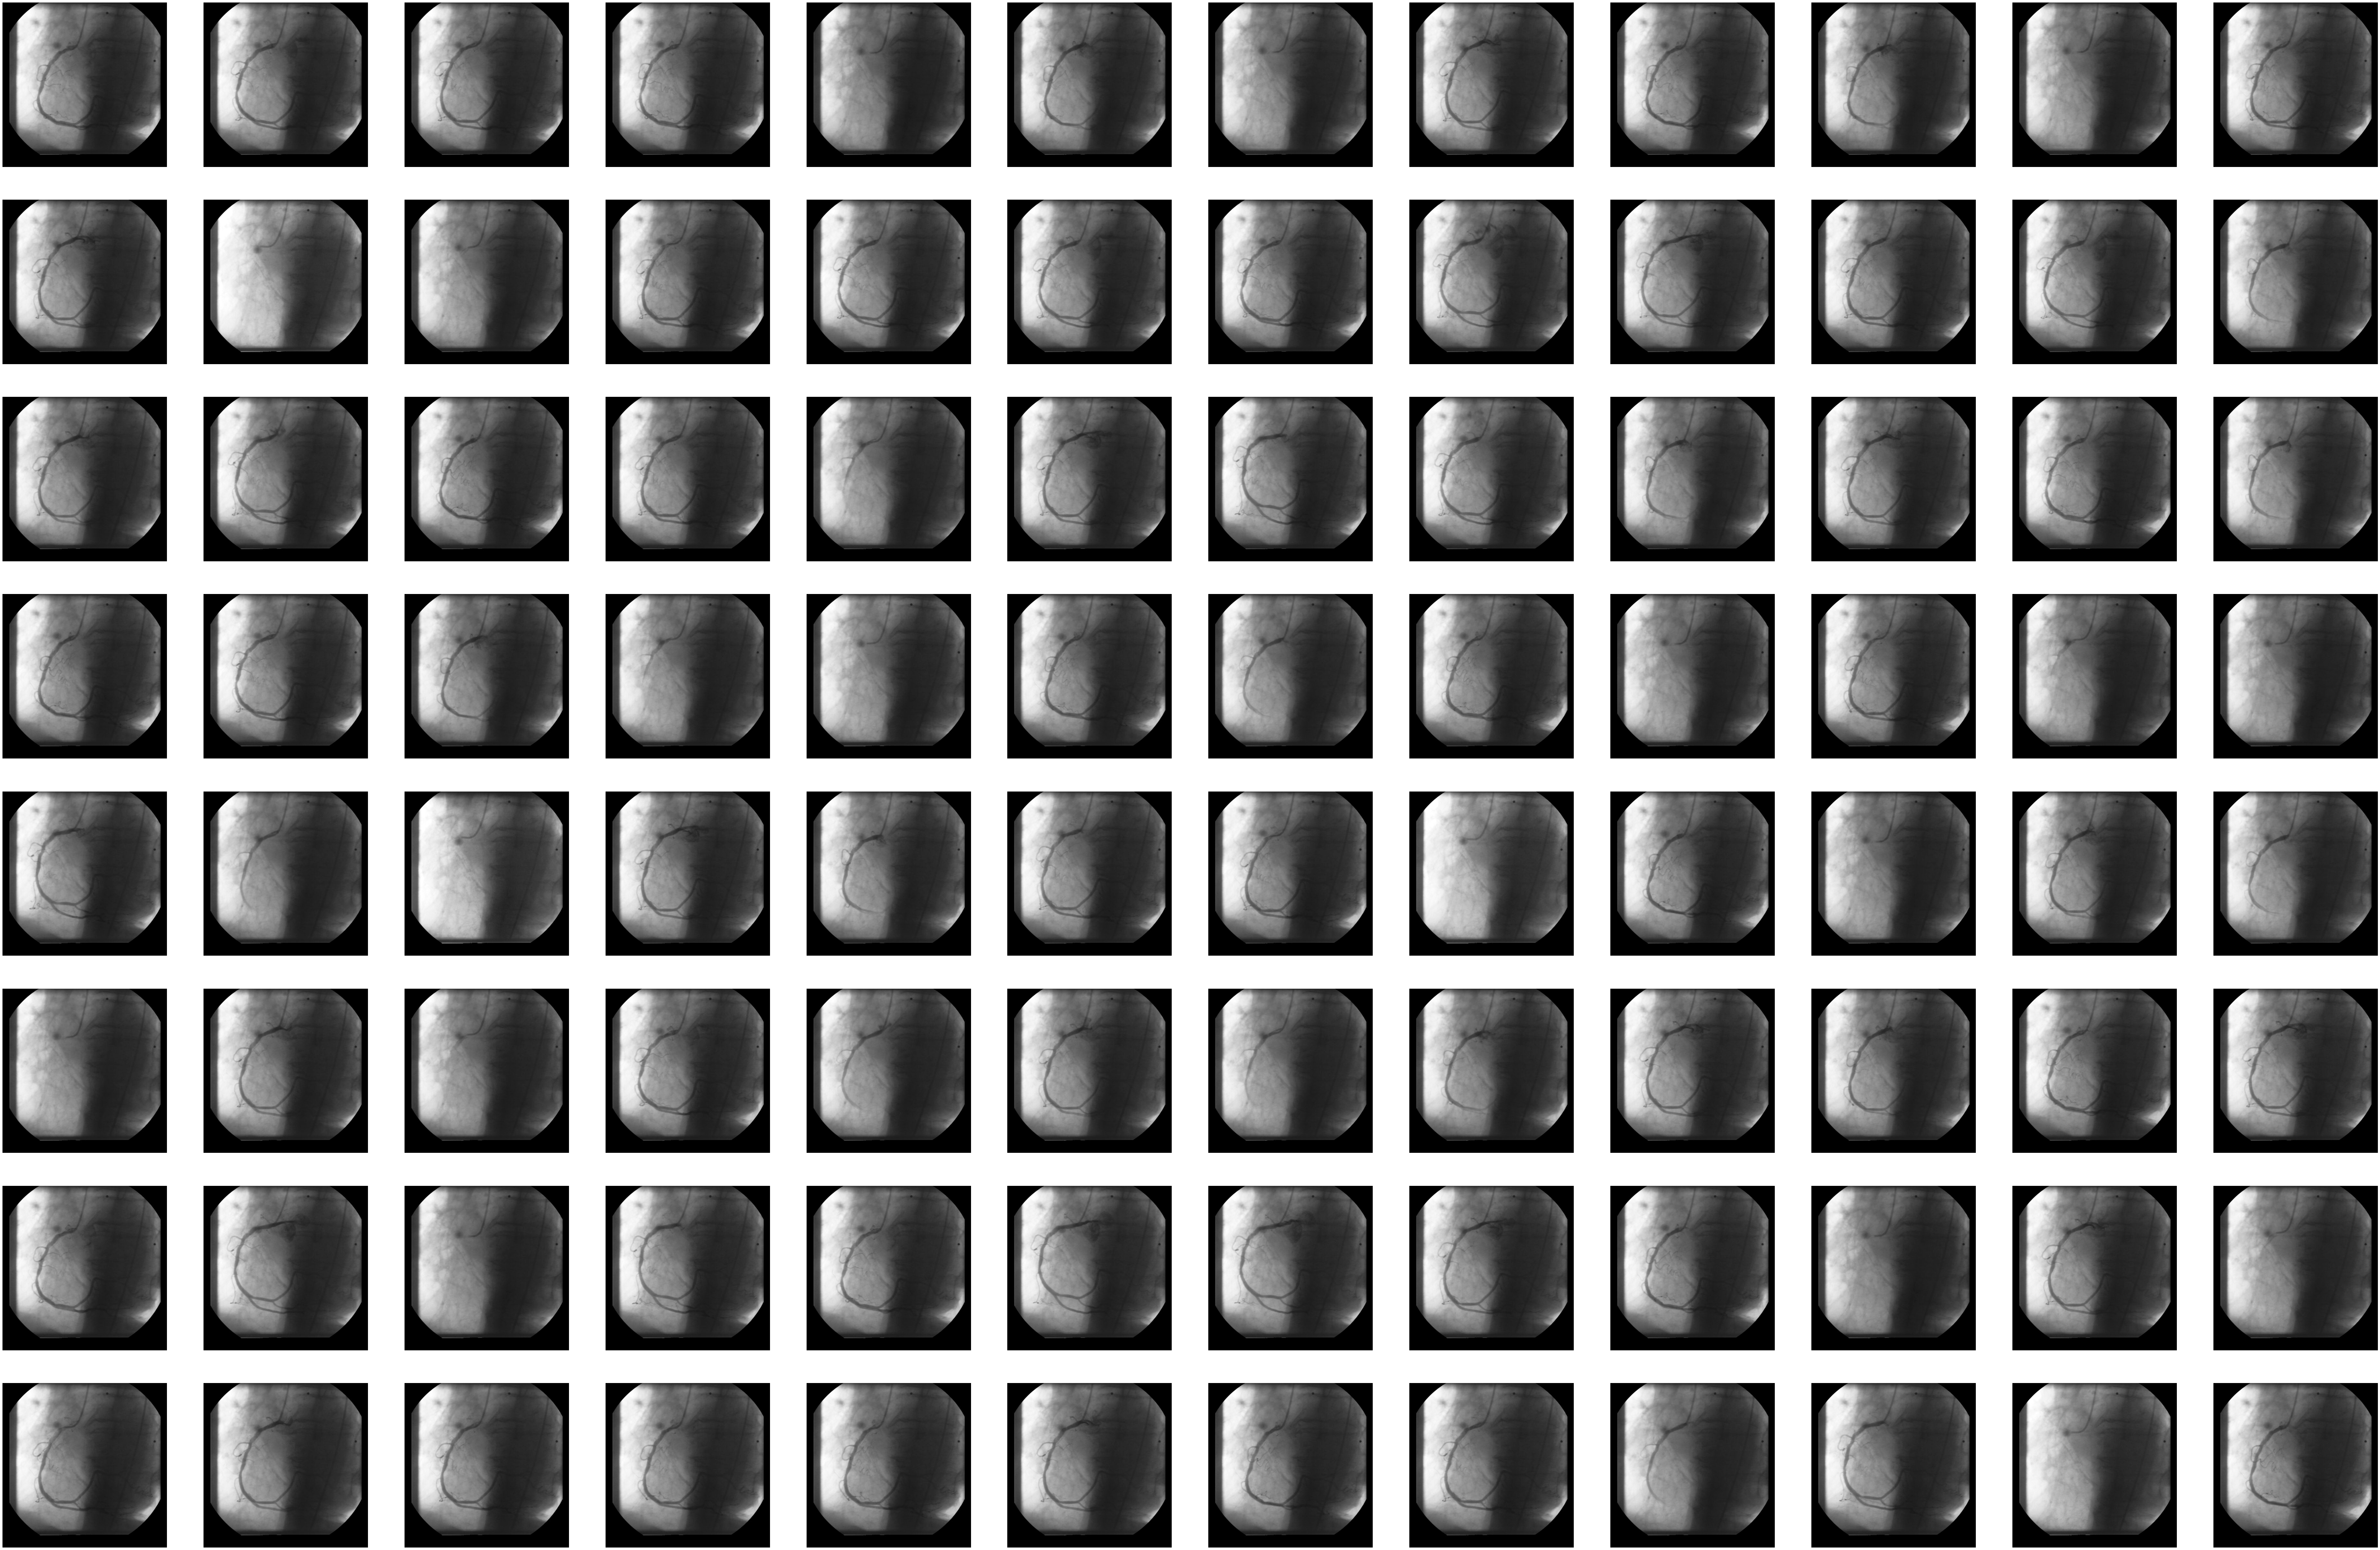
\includegraphics[width=14cm]{fig/images_in_dicom.png}
    \legend{Fonte: Autor com imagens do \cite{cancer_imaging_archive_cancer_2022}.}
    \label{fig:fig21}
\end{figure}

Outro ponto do código contido na imagem \ref{fig:fig18} que deve ser explicado, são as linhas 11 e 12. Para salvar as imagens em um formato comum, é necessário converter seus pixeis para o valor correto. Por padrão as imagens contém pixeis com valores entre 0 e 255 e é isso que a linha 11 faz: normaliza os pixeis para um valor entre 0 e 255. E por fim, a linha 12 converte cada pixel para um inteiro de 8 bits.

Agora, a imagem está em um formato utilizável para treinar o modelo. Para fazer este procedimento em todas as imagens da base, o programa precisa ser alterado para ler os arquivos \textit{DICOM} do disco de forma automática e escrever os novos arquivos \textit{jpg} também de forma automatizada.

\subsection{Uniformização e redução da resolução}
\label{sec:uniformizacao}

Um dos requisitos necessários para se treinar o modelo é uma resolução uniforme em todas as imagens. Uniforme em alguns aspectos: largura e altura consistentes e ambas as dimensões devem ser múltiplas de \textbf{N}, onde \textbf{N} é a escala na qual o modelo será treinado para performar. \textbf{N} vale 4 para o contexto deste trabalho, já que o modelo treinado, será capaz de super resolver imagens em quatro vezes o tamanho original.

Não é necessário preocupar com a consistência entre largura e altura já que as imagens originalmente possuem altura e largura uniformes em todas as imagens selecionadas para treinamento. A segunda parte contudo, há de ser feita.

Transformar todas as milhares de imagens em imagens com resoluções múltiplas de 4 manualmente é uma tarefa completamente infactível. Alguma forma de automação deste processo é indispensável para a continuação do trabalho. Foi considerado o desenvolvimento de um software para tal, que fosse capaz de ler imagens do disco, encontrar sua resolução e redimensiona-la para o valor mais próximo que também fosse múltiplo de 4. O desenvolvimento e testes de tal ferramenta demandaria bastante tempo para ser implementado e testado. Se levada em consideração, a necessidade de que este software seja flexível à novas configurações (como novos valores para \textbf{N}, por exemplo), novas operações (como cortes em imagens, por exemplo), é razoável concluir com boa precisão, que ainda mais tempo seria desprendido para trabalhar na criação de uma ferramenta capaz de realizar todas estas tarefas.

Este desenvolvimento foi dispensado, pois um software de código aberto chamado \textit{Magick-Utils} não muito famoso, já faz a conversão da resolução de forma automatizada. Este software foi encontrado de forma inesperada, na descrição de um vídeo tutorial para o treinamento de uma implementação do modelo ESRGAN, e seu código é completamente aberto

\begin{figure}[H]
    \centering
    \caption{Captura de tela do software \textit{Magick-Utils}.}
    \includegraphics[width=14cm]{fig/magick-utils.png}
    \legend{Fonte: \textit{Github} do criador do software \cite{n00mkrad_magickutils_2022}. }
    \label{fig:fig22}
\end{figure}

O processo é relativamente lento, mas é possível fazer a conversão de todas as imagens em algumas horas.

Como descrito na seção \ref{sec:prep-imgs}, uma das formas de se controlar tempo e consumo de recursos do treinamento é reduzindo a resolução das imagens. Caso tal redução se faça necessária, o software \textit{Magick-Utils} \cite{n00mkrad_magickutils_2022} é perfeito para a tarefa. O programa suporta o usuário selecionar uma pasta inteira contendo dezenas de milhares de imagens. Este, irá alterar todas as imagens para uma resolução menor, até que as imagens estejam em um tamanho praticável para os recursos computacionais disponíveis para o treinamento.

\section{Considerações gerais sobre as imagens pós processadas}
\label{sec:desenvolvimento:general-considerations-post-processed-images}

Para sumarizar o estado das bases de imagens após o processamento descrito nas seções anteriores, segue a tabela abaixo:

\begin{table}[H]
    \centering
    \caption{Tabela sumarizando as imagens processadas.}
    \begin{tabular}{|l|l|l|} \hline
        \multirow{2}{*}{\textbf{Estatística}}   & \multicolumn{2}{|c|}{\textbf{Base de imagens}}            \\ \cline{2-3}
                                                & \textbf{Ressonância magnética}    & \textbf{Astronomia}   \\ \hline
        \textbf{Nº de imagens}                  & 6031                              & 243435                \\ \hline
        \textbf{Resolução}                      & 108x108                           & 424x424               \\ \hline            
        \textbf{Tamanho médio (bytes)}          & 4288.04                           & 12674.51              \\ \hline            
        \textbf{Tamanho 90º percentil (bytes)}  & 5314.6                            & 17674.51              \\ \hline            
        \textbf{Cor}                            & Monocromática (Tons de cinza)     & Colorida              \\ \hline            
    \end{tabular}
    \vspace{0.3cm}
    \legend{Fonte: Autor.}
    \label{tab:image_considerations}
\end{table}

Algumas das diferenças entres as bases de dados podem impactar no treinamento. A resolução das imagens astronômicas é quase quatro vezes maior que a resolução das imagens médica e em consequência, também medem mais de três vezes mais em disco.

Como se a diferença de resolução não bastasse, as imagens astronômicas são coloridas. A presença de cor aumenta, em algumas dimensões a estrutura de dados, neste caso, o tensor que irá trafegar nas redes. Enquanto uma imagem monocromática como as da base médica, pode ser representada com uma estrutura bidimensional. A imagem colorida requer mais uma dimensão para os canais de cores.

\begin{figure}[H]
    \centering
    \caption{Diagrama demonstrando diferença estrutural entre imagem monocromática e colorida.}
    \includegraphics[width=12cm]{fig/monochrome_vs_color.png}
    \legend{Fonte: Autor}
    \label{fig:monochrome_vs_color}
\end{figure}

Na figura \ref{fig:monochrome_vs_color}, a imagem A representa uma imagem monocromática, com apenas duas dimensões: altura e largura. A imagem B, representa uma imagem colorida com cores RGB. Uma dimensão a mais é necessária para armazenamento e processamento: os canais de cores.

\section{Preparação do ambiente para treinamento}
\index{Treinamento}
\label{sec:environment-prep-training}


Nesta parte do trabalho, é descrita toda a configuração, e tentativas de configuração, necessárias para o treinamento correto do modelo ESRGAN. Detalhes do hardware disponível e utilizado são apresentados, assim como também especificações de software como sistema operacional, bibliotecas utilizadas, forma de executar o treinamento etc.

O modelo utilizado, consiste em uma implementação de terceiros da especificação da ESRGAN já que entender os pormenores deste modelo é um esforço muito além do escopo do trabalho. Como utilizar tal software, envolve lidar com softwares e implementações externos, é preciso ater-se aos detalhes disponibilizados para que seja possível configurar o ambiente e preparar as entradas de forma correta.

Antes da descrição mais acurada do processo, é fundamental deixar claro os requisitos necessários para utilizar uma ESRGAN. O modelo, como explicado anteriormente consiste de várias camadas de processamento. Cada uma destas, executa uma quantidade significativa de cálculos cada vez que o modelo é alimentado com dados de entrada, seja em fase de treinamento, testes ou na utilização real.

Modelos como este, assim como diversos outros tipos de modelos de inteligência artificial, conseguem tirar bastante proveito de processadores com vários núcleos. Estes processadores conseguem, quando implementado de tal forma, realizar uma grande quantidade de cálculos simultaneamente. Cálculos que individualmente são simples operações matemáticas, mas quando combinados da forma correta, representam todo o modelo que este trabalho analisa. Um tipo de processador que se encaixa nesta categoria, são as GPUs (Graphics Processing Unit, unidade de processamento de gráficos, do inglês).\index{GPU} Vários dispositivos domésticos vêm de fábrica com uma GPU dedicada que possui centenas, senão milhares de núcleos.

Com isso em mente, diversos modelos e bibliotecas de computação numérica e inteligência artificial são desenvolvidos com a ideia de que serão treinadas, testadas e utilizadas em GPUs, em mente. Vários testes de performance demonstram a superioridade das GPUs em comparação com os processadores tradicionais (CPUs)\index{CPU} para tarefas de treinamento de modelos de inteligência artificial. De acordo com \citeonline{pantigoso_velasquez_performance_2019}, para modelos mais complexos é notável a diferença de desempenho quando se utiliza de GPUs para o treinamento. Esta diferença no entanto, decresce com modelos mais simples.

Para usufruir deste hardware, é necessário no entanto de uma forma de interface para que o modelo, implementado utilizando uma tecnologia \textbf{X}, representando qualquer variação do modelo feito com tecnologias distintas, possa acessar os recursos da GPU, independente do modelo. É esse o papel do CUDA. Uma ferramenta desenvolvida pela \textit{NVIDIA} para fazer esse interfaceamento. CUDA, de acordo com a própria empresa por trás da ferramenta, é uma plataforma de computação paralela que engloba diversos recursos. A ferramenta é capaz de compilar código para executar em GPUs, usar interfaces em diferentes linguagens para acessar recursos do hardware entre outras coisas. Os desenvolvedores que utilizam CUDA, determinam quais partes do código devem ser executadas de forma paralela e demarcam este trecho com anotações. O compilador ou interpretador então, detecta estes trechos e os executa em núcleos paralelos na GPU.

Várias destas bibliotecas utilizadas para desenvolver modelos de inteligência artificial e redes neurais fazem uso de recursos matemáticos como tensores, que generalizam várias estruturas básicas: valores escalares, vetores, matrizes etc. Existem hardwares específicos para processamento de tensores, os assim chamados TPUs (Tensor Processing Unit, unidade de processamento de tensores, do inglês) e inclusive, há formas de acessá-los de forma gratuita. Como o modelo utilizado neste trabalho foi desenvolvido e otimizado para GPUs, é supérfluo entrar em mais detalhes sobre TPUs. Vale no entanto, a menção e talvez um trabalho futuro envolvendo o assunto.\index{TPU}

\subsection{Descrevendo o hardware disponível}
\index{Treinamento}

Para treinar o modelo, um computador esteve disponível. A especificação de seu hardware está contida na tabela abaixo:

\begin{table}[H]
    \centering
    \caption{Tabela de descrição do hardware}
    \begin{tabular}{|l|l|} \hline
        \textbf{Item}            & \textbf{Descrição}                    \\ \hline
        CPU                      & Intel i7 Octa Core                    \\ \hline
        Memória RAM              & 16GB                                  \\ \hline
        Memória de Vídeo         & 2GB                                   \\ \hline
        Modelo da placa de vídeo & GeForce MX350                         \\ \hline
        Disco                    & 512GB (apenas 90GB disponível)        \\ \hline
        Sistema operacional      & Windows 10 e Ubuntu 24.04 disponível  \\ \hline
    \end{tabular}
    \vspace{0.3cm}
    \legend{Fonte: Autor.}
    \label{tab:my_label}
\end{table}

A placa de vídeo apresentada (GeForce GT920M) é um modelo de computadores portáteis voltada para jogos. Uma informação importante de se documentar, é sua quantidade de Núcleos \textit{CUDA}\index{CUDA} conhecidos popularmente pelo termo em inglês \textit{Cuda Core}. Os núcleos \textit{CUDA} são os núcleos de processamento de instruções das \textit{GPUs} da \textit{NVIDIA}, conceito bem parecido com o conceito de núcleos de processadores \cite{ryles_what_2022}. A placa em questão possui compatibilidade com \textit{CUDA}, um requisito indispensável, e possui 384 núcleos \textit{CUDA} \cite{nvidia_geforce_2022, technical_city_nvidia_2022}. Esta placa de vídeo de entrada possui 96 vezes mais núcleos que a CPU disponível.

O hardware descrito, está distante de ser o ideal para o treinamento de um modelo complexo e exigente em termos de recursos, como é o caso do modelo descrito e utilizado neste trabalho. Treinamentos do tipo costumam ser feitos em servidores dedicados, com processadores poderosos e grandes quantidades de memória RAM e memória de vídeo (VRAM).

Por causa desta limitação de recursos, é preciso recorrer à alternativas a nível de software, como descrito na seção \ref{sec:prep-imgs}.


\subsection{Descrição do software necessário para treinar o modelo}

Para treinar, executar e utilizar o modelo de forma geral, as dependências da implementação utilizada devem ser satisfeitas. Ou seja, é preciso antes, instalar as bibliotecas, \textit{frameworks} etc. necessários para a execução do modelo.

Nesta seção será descrito, com o maior nível de detalhes possível, como este processo é realizado. Da preparação do ambiente até à execução do treinamento e do modelo em si. Tenha em mente que esta etapa, apesar de parecer simples (afinal, consiste apenas em instalar softwares e no máximo fazer uma eventual configuração), pode ser bastante complicada por alguns motivos.

O primeiro passo nesta tarefa é reproduzir o ambiente onde o modelo foi desenvolvido e testado. Reproduzir um ambiente qualquer, requer manter todas as bibliotecas e softwares em geral, na mesma versão que o ambiente desejado, ou pelo menos manter tudo em uma versão compatível. Caso o(s) desenvolvedor(es) do modelo forneçam estas informações, grande parte do esforço está adiantado. Caso estas informações não estejam disponíveis, estas precisam, de forma não negociável, ser encontradas, seja buscando em fóruns ou outras fontes elaboradas por pessoas que passaram pelo mesmo problema, ou por tentativa e erro.

O segundo motivo complicador desta fase do trabalho, é a compatibilidade entre software e hardware. Como explicado anteriormente, reproduzir o ambiente a nível de software requer encontrar uma interseção de compatibilidade entre todas as dependências necessárias para executar o modelo. O mesmo acontece com hardware. Alguns dispositivos, como \textit{GPUs}, que são extremamente necessárias para este trabalho, possuem \textit{drivers} específicos em versões específicas, que integram com versões particulares de bibliotecas necessárias. Até aí, nenhuma novidade em relação aos problemas de software. Quando tratamos de hardware no entanto, não se pode contar com versões atualizadas de determinado \textit{driver} para sempre. Os desenvolvedores podem interromper o suporte de uma \textit{GPU} A, mais antiga e obsoleta, para concentrarem os esforços num modelo B, mais atualizado. Isto pode ser um problema comprometedor, especialmente quando há uma limitação tão grande de hardware como é o caso deste trabalho.

\subsubsection{Experimentos preliminares com o ambiente}

Os primeiros experimentos de preparação do ambiente foram feitos em um computador com uma instalação do sistema operacional Ubuntu versão 18.04LTS. Várias fontes informais como vídeos e comentários em fóruns e redes sociais sobre o assunto recomendaram o uso de uma distribuição Linux qualquer para o treinamento de modelos complexos e pesados como o modelo atual. As recomendações sempre levavam em consideração a forma como os sistemas operacionais Linux gerenciam os recursos de forma mais minimalista, deixando mais memória, processador e disco disponíveis para o treinamento em si. Além disso, Linux pareceu uma boa primeira alternativa, devido à familiaridade de uso.

Contudo, os experimentos no Linux foram um insucesso. Como parte das dependências são fornecidas pela empresa \textit{NVIDIA}, suas bibliotecas proprietárias precisam ser instaladas no Linux e isso nem sempre é uma tarefa simples. No experimento realizado, ao instalar o \textit{driver} necessário para utilizar a \textit{GPU}, várias funcionalidades básicas do sistema operacional pararam de funcionar propriamente.

Como uma instalação do Windows 10 estava disponível, não valeria o esforço de tentar resolver os diversos problemas de compatibilidade entre dependências da \textit{NVIDIA} e o sistema operacional, o desenvolvimento prosseguiu utilizando como sistema operacional, o Windows 10.

\subsubsection{Breve descrição sobre versões}
\label{sec:environment-version-compatability}

Para fazer qualquer procedimento com este modelo, seja treinamento, teste ou execução, vários níveis de compatibilidade de software com software e de software com hardware precisam ser garantidos. O diagrama abaixo ilustra a interação entre as partes:

\begin{figure}[H]
    \centering
    \caption{Diagrama de interação entre as partes envolvidas no modelo.}
    \includegraphics[width=14cm]{fig/version_diagram.png}
    \legend{Fonte: Autor.}
    \label{fig:fig24}
\end{figure}

Na figura \ref{fig:fig24}, os blocos laranja fazendo contato entre si representam compatibilidade de comunicação entre as partes. Ao todo são quatro níveis de compatibilidade. As versões do \textit{python} e dos frameworks (\textit{PyTorch} e \textit{Tensorflow}) já são predeterminadas pela implementação do modelo. A dificuldade vem em encontrar uma versão do CUDA que se comunica com a versão dos frameworks e do \textit{driver} e uma versão do \textit{driver} que se comunica com o hardware em si.

\subsubsection{Instalação do \textit{driver} da \textit{NVIDIA}}
\label{sec:driver}
\index{NVIDIA}
\index{GPU}

O passo base para prosseguir com a instalação das dependências, é instalar um \textit{driver} compatível com ambos, a placa de vídeo disponível, e a versão das bibliotecas utilizadas.

Esta seção, apesar de ter sido colocada imediatamente anterior à seção sobre \textit{CUDA}\index{CUDA} (vide seção \ref{sec:cuda}) devido à ordem cronológica correta e esperada dos passos, foi desenvolvida em repetição antes e após a instalação do \textit{CUDA}. Isto aconteceu por inúmeros problemas de compatibilidade que apareceram ao tentar integrar o \textit{driver} com a biblioteca e estes dois com o hardware em si. O processo é extremamente demorado e mecânico. Como a instalação e desinstalação tomam bastante tempo por si só, é de se esperar que fazê-los várias vezes até obtermos uma combinação compatível entre si, tomaria muito tempo.

Para encontrar o \textit{driver} específico ao \textit{hardware} (GPU) disponível, basta buscar no mecanismo oficial de busca de \textit{drivers} atualizados do site da \textit{NVIDIA} (figura \ref{fig:fig23}).

\begin{figure}[H]
    \centering
    \caption{Captura de tela do buscador de drivers da \textit{NVIDIA}.}
    \includegraphics[width=14cm]{fig/nvidia_driver.png}
    \legend{Fonte: Buscador de \textit{drivers} atualizados da \textit{NVIDIA} \cite{nvidia_download_2023} }
    \label{fig:fig23}
\end{figure}

Caso, por motivos de compatibilidade o \textit{driver} atualizado não integre com as bibliotecas necessárias para o desenvolvimento, existe ainda a alternativa de procurar por versões anteriores ou versões de teste do \textit{driver} para o hardware. A figura \ref{fig:fig24} mostra o buscador avançado de \textit{drivers} que a \textit{NVIDIA} disponibiliza. Nele, dispõe-se várias opções com as quais é possível experimentar. Basta buscar pelo modelo do seu hardware, filtrando pelas várias opções disponíveis.

\begin{figure}[H]
    \centering
    \caption{Captura de tela do buscador avançado de drivers da \textit{NVIDIA}.}
    \includegraphics[width=14cm]{fig/nvidia_driver_advanced.png}
    \legend{Fonte: Buscador avançado de \textit{drivers} da \textit{NVIDIA} \cite{nvidia_advanced_2023} }
    \label{fig:nvidia-site:fig24}
\end{figure}

Após encontrar o \textit{driver} específico, basta fazer o \textit{download}, executar o arquivo e seguir os passos para instalação. A instalação contém várias opções e componentes mais voltadas para cenários específicos. As opções padrão geralmente são suficientes para a maior parte dos casos, de acordo com os testes realizados. Além da instalação do \textit{driver}, algumas atualizações podem ser necessárias. O instalador é capaz de resolvê-las por conta própria.

\subsubsection{Instalação do CUDA}
\label{sec:cuda}
\index{CUDA}
\index{NVIDIA}

Esta parte precisa de ser realizada em perfeita harmonia com a seção \ref{sec:driver}. Qualquer versão incorreta pode impedir o funcionamento do projeto como um todo.

A primeira parte da instalação, como esperado, é baixar o instalador. Isso pode ser feito através do site da \textit{NVIDIA Developers}. Um site voltado para usuários mais técnicos que desenvolvem para as plataformas da \textit{NVIDIA}.

\begin{figure}[H]
    \centering
    \caption{Captura de tela do site da \textit{NVIDIA Developers}.}
    \includegraphics[width=12cm]{fig/cuda_download_page.png}
    \legend{Fonte: Buscador de instaladores CUDA \cite{nvidia_cuda_2024}. }
    \label{fig:fig25}
\end{figure}

A figura \ref{fig:fig25} mostra a página inicial do site. Para encontrar o instalador correto para cada situação, preencha o filtro com os detalhes desejados.

\begin{figure}[H]
    \centering
    \caption{Captura de tela do filtro do buscador de instaladores CUDA.}
    \includegraphics[width=12cm]{fig/cuda_download_page_installer_type.png}
    \legend{Fonte: Filtros do buscador de instaladores CUDA \cite{nvidia_cuda_2024}. }
    \label{fig:fig26}
\end{figure}

Com os filtros da figura \ref{fig:fig26} preenchidos, serão disponibilizadas duas versões para download (\textit{Installer type}, tipo do instalador, do inglês): o instalador completo (opção \textit{local}) e o instalador pela rede (opção \textit{network}). O instalador completo faz um download lento e grande mas uma vez baixado, nenhum download extra será necessário. O segundo, pela rede, baixa um instalador mais compacto e, durante a instalação faz o download do restante. Ambas opções trarão o mesmo resultado. Após a escolha do tipo de instalador, um botão para o download será exibido.

\begin{figure}[H]
    \centering
    \caption{Captura de tela da busca de instaladores CUDA.}
    \includegraphics[width=10cm]{fig/cuda_download_page_final.png}
    \legend{Fonte: Busca completa de instaladores CUDA \cite{nvidia_cuda_2024}. }
    \label{fig:fig27}
\end{figure}

Faça o download, clicando no botão destacado na figura \ref{fig:fig27} e execute o arquivo baixado.

\index{CUDA}
\begin{figure}[H]
    \centering
    \caption{Captura de tela de instalação CUDA.}
    \includegraphics[width=10cm]{fig/cuda_instalacao.png}
    \legend{Fonte: Tela do instalador CUDA. \cite{kitson_installing_2022}}
    \label{fig:fig28}
\end{figure}

Nas opções do instalador acima, serão disponibilizadas a versão expressa e a versão avançada. A versão expressa, de instalação mais rápida, é suficiente para o propósito desta instalação. Siga os passos normalmente até finalizar. Esta instalação pode tomar um tempo considerável, dependendo do tipo de instalador escolhido. Caso a opção rede (\textit{network}) tenha sido a escolhida, a maior parte do software será baixada durante a instalação, justificando assim a demora extra.

\subsection{Apresentação do modelo}

Nesta subseção, detalhes sobre a implementação do modelo, assim como características de configurações serão descritos.

\subsubsection{Descrevendo a implementação}

Algumas implementações foram utilizadas durante os experimentos. Cada uma delas, fornece uma abordagem diferente para a mesma arquitetura, apesar de compartilharem o mesmo objetivo final. Uma das principais diferenças encontradas entre implementações distintas, são as ferramentas utilizadas para desenvolvê-las. Sejam versões diferentes ou ferramentas completamente diferentes.

O requisito necessário para que uma destas implementações sejam adequadas para o trabalho é interoperabilidade com os drivers e hardwares disponíveis. No final das contas, as implementações utilizadas podem ser divididas em dois grupos:

\begin{itemize}
    \item Modelos implementados utilizando a biblioteca \textit{Tensorflow}
    \item Modelos implementados utilizando a biblioteca \textit{PyTorch}
\end{itemize}

Ambas as bibliotecas são extremamente populares no meio científico de aprendizado de máquinas e computação numérica em geral. Estas bibliotecas abstraem parte da complexidade matemática por trás das construções e execuções dos modelos, dando à pessoa que está desenvolvendo, uma linguagem mais declarativa e de alto nível para expressar suas intenções. Toda a parte algébrica por trás do modelo, é então trabalhada pela biblioteca. Otimizações e transformações são feitas, para maximizar o aproveito do hardware, livrando assim, o(a) desenvolvedor(a) final de tais aperfeiçoamentos.

Após várias tentativas com modelos baseados no Tensorflow, foi concluído que, dado o recurso computacional disponível, estes modelos não iriam trazer resultados satisfatórios em tempo hábil. Os treinamentos com os modelos em Tensorflow testados, produziam erros de memória insuficiente para treinamento, horas após o início do processo.

Treinar as redes só foi possível com os modelos em Tensorflow utilizados, quando os parâmetros de treinamentos eram absurdamente baixos (e.g. uma imagem carregada por vez, i.e. um \textit{batch\_size} de 1). Isso por si só iria deteriorar consideravelmente a qualidade dos resultados, dentro do tempo disponível para treinamento que inicialmente, compreendia o período noturno, quando a máquina não estava sendo utilizada. Ou seja, os modelos baseados no Tensorflow iriam tomar um tempo impraticável para atingir um número \textbf{n} de épocas.

Além disso, nem todos os modelos em Tensorflow eram executáveis na máquina utilizada, seja por incompatibilidade de versões das bibliotecas, seja por erros de configuração. 

No final das contas, um modelo baseado em PyTorch foi o escolhido. Este modelo possui certa complexidade para se configurar, mas diferente dos modelos em Tensorflow testados anteriormente, as falhas acontecem cedo, permitindo assim melhor adaptabilidade no treinamento. O consumo de memória deste modelo, também foi significativamente menor, com parâmetros pequenos (mas não tão pequenos a ponto de delongar muito o treinamento), é possível utilizar a máquina para outras tarefas paralelas, algo infactível nos modelos anteriores. 

O modelo de código aberto \textit{BasicSR} \cite{blueamulet_blueamuletbasicsr_2023}, foi o modelo eleito. O projeto em si, contém outras implementações e capacidades, mas para o escopo desse trabalho, o foco principal foi sob o módulo de ESRGAN com super resolução de quatro vezes das imagens de entrada. A implementação é baseada no modelo de ESRGAN anteriormente citado neste trabalho \cite{wang_esrgan_2018}.


\subsubsection{Detalhando a preparação do projeto para treinamento}
\label{sec:preping-project-for-training}

Para executar a implementação, seja treinamento ou execução, esta antes, deve ser configurada. O projeto utilizado requer duas configurações básicas além obviamente, das dependências descritas anteriormente (driver da NVIDIA e CUDA). Primeiramente um modelo pré-treinado inicial deve ser encontrado assim como um arquivo de configurações contendo os dados que o modelo precisa para funcionar propriamente, como caminho para o diretório com os dados de treinamento, qual algoritmo de treinamento utilizar, etc.

Os modelos pré-treinados podem ser encontrados juntos com o projeto da implementação do modelo. Uma característica muito importante que deve ser levada em consideração é a arquitetura do modelo pré-treinado. Essa arquitetura deve ser idêntica à arquitetura para a qual o modelo irá ser treinado, ou seja, se uma ESRGAN para fazer super resolução de quatro vezes será treinada, obrigatoriamente, um modelo pré-treinado de ESRGAN com super resolução de quatro vezes deve ser utilizado. Qualquer outra variação não irá funcionar, devido à falta de compatibilidade da estrutura interna das camadas e pesos entre uma arquitetura e outra.

Após obtido o modelo pré-treinado, deve se organizar os dados de treinamento de uma maneira específica para que a implementação possa entender e configurar o projeto. Como o objetivo é obter um modelo treinado capaz de super resolver imagens em quatro vezes sua resolução inicial, as bases de dados devem estar dispostas com as seguintes características:

\begin{enumerate}
    \item Uma base de dados de treinamento, contendo:
    \begin{itemize}
        \item Imagens em baixa resolução 
        \item A versão de alta resolução (quatro vezes a resolução) das imagens de baixa resolução
    \end{itemize}
    \item Uma base de dados de validação, contendo:
    \begin{itemize}
        \item Imagens em baixa resolução
        \item A versão de alta resolução (quatro vezes a resolução) das imagens de baixa resolução
    \end{itemize}
\end{enumerate}

A proporção de dados separados para cada uma das duas bases de dados foi de 80:20: 80\% das imagens dedicadas à treinamento, e 20\%, dedicadas à validação. Para gerar as imagens de baixa resolução, a partir das imagens de alta resolução, o processo descrito na seção \ref{sec:uniformizacao} foi utilizado. 

Com as imagens preparadas e distribuídas em diretórios específicos, de acordo com a descrição anterior, os caminhos onde cada uma das divisões da base de dados se encontra podem ser adicionados no arquivo de configuração do projeto.

\begin{figure}[H]
    \centering
    \caption{Trecho do arquivo de configuração para treinamento e execução da implementação do modelo.}
    \includegraphics[width=12cm]{fig/carbon_configuracao_basic_sr.png}
    \legend{Fonte: Autor.}
    \label{fig:fig29}
\end{figure}

No arquivo de configuração mostrado anteriormente, alguns parâmetros devem ter atenção especial. O parâmetro \textit{scale} representa a proporção na qual deseja-se treinar o modelo, quatro nesse caso. Os parâmetros \textit{dataroot\_HR} e \textit{dataroot\_LR} representam o diretório com as imagens de alta e baixa resolução, respectivamente, para treino e validação. E por último, mas não menos importante, o atributo \textit{pretrain\_model\_G} é o caminho onde está armazenado o modelo pré-treinado.


\subsection{Descrição dos experimentos práticos de treinamento}

O processo anterior foi feito a partir do zero para duas bases de imagens diferentes, criando uma cópia do projeto no final do processo por segurança. Desta forma, os resultados do modelo terão uma maior reprodutibilidade.

\subsubsection{Executando o modelo}

Com tudo configurado e preparado, basta executar o modelo, com o comando abaixo, seguindo as opções recomendadas na documentação do projeto:

\begin{figure}[H]
    \centering
    \caption{Comando para executar o treinamento.}
    \includegraphics[width=12cm]{fig/carbon_executar_projeto.png}
    \legend{Fonte: Autor.}
    \label{fig:fig30}
\end{figure}

Estes parâmetros utilizados acima, foram os que funcionaram melhor após experimentar com o modelo. Perceba, que o \textit{batch\_size} é 2, assim como no projeto em Tensorflow mencionado anteriormente. No caso anterior, treinar com apenas duas imagens por vez era um impeditivo, dada a extensão no tempo total do treinamento. Com este modelo atual no entanto, em cerca de dez horas o treinamento cobria próximo de 100 épocas com 1000 iterações cada. Um número razoável para o propósito do trabalho. 


\section{Coleta de dados}

Nesta seção, será descrito o procedimento pelo qual a colheita de dados foi feita. Diversas automações foram feitas para extrair o máximo de dados com o mínimo de tempo. Quanto mais dados coletados, mais rica é a analise.

\subsection{Experimentos de similaridade entre imagens}
\label{sec:experimentos-similaridade-imagens}

Como dito na seção \ref{sec:qualidade-imagem}, existem formas quantitativas de avaliar a qualidade de imagens. Um pequeno programa foi desenvolvido para lidar com essa tarefa de forma automatizada \cite{vasconcelos_leonamtvimage-similarity-scripts_2023}. O programa executa em linha de comando, recebendo como parâmetros as duas imagens e os algoritmos de similaridade que será utilizado. O software tem os seguintes algoritmos de similaridade disponíveis: MSE, RMSE, PSNR, UQI, SSIM, ERGAS, SCC, RASE, SAM, MSSSIM e VIFP.

Para o escopo deste trabalho, serão utilizados os algoritmos MSE, RMSE, PSNR e ERGAS. A sintaxe utilizada segue o seguinte padrão

\begin{figure}[H]
    \centering
    \caption{Diagrama de sintaxe do programa.}
    \includegraphics[width=14cm]{fig/similarity/image_similarity_script.png}
    \legend{Fonte: Autor.}
    \label{fig:fig31}
\end{figure}

Na figura \ref{fig:fig31}, o parâmetro \textit{algoritmo} representa quais algoritmos serão utilizados para calcular a similaridade entre as imagens. para executar todos os algoritmos, deve-se passar uma lista com todos os desejados, ou passar o parâmetro \textit{--all}.

Para alimentar o programa com as imagens, os parâmetros \textit{--img\_a} e \textit{--img\_b} são utilizados. Estes recebem os caminhos das imagens. O parâmetro \textit{--verbose}, caso passado, imprime algumas informações a mais.

\subsubsection{Exemplo de execução do programa acima}

Para o exemplo, as duas imagens abaixo serão utilizadas:

\begin{figure}[H]
    \centering
    \caption{Imagem A e imagem B utilizadas no teste.}
    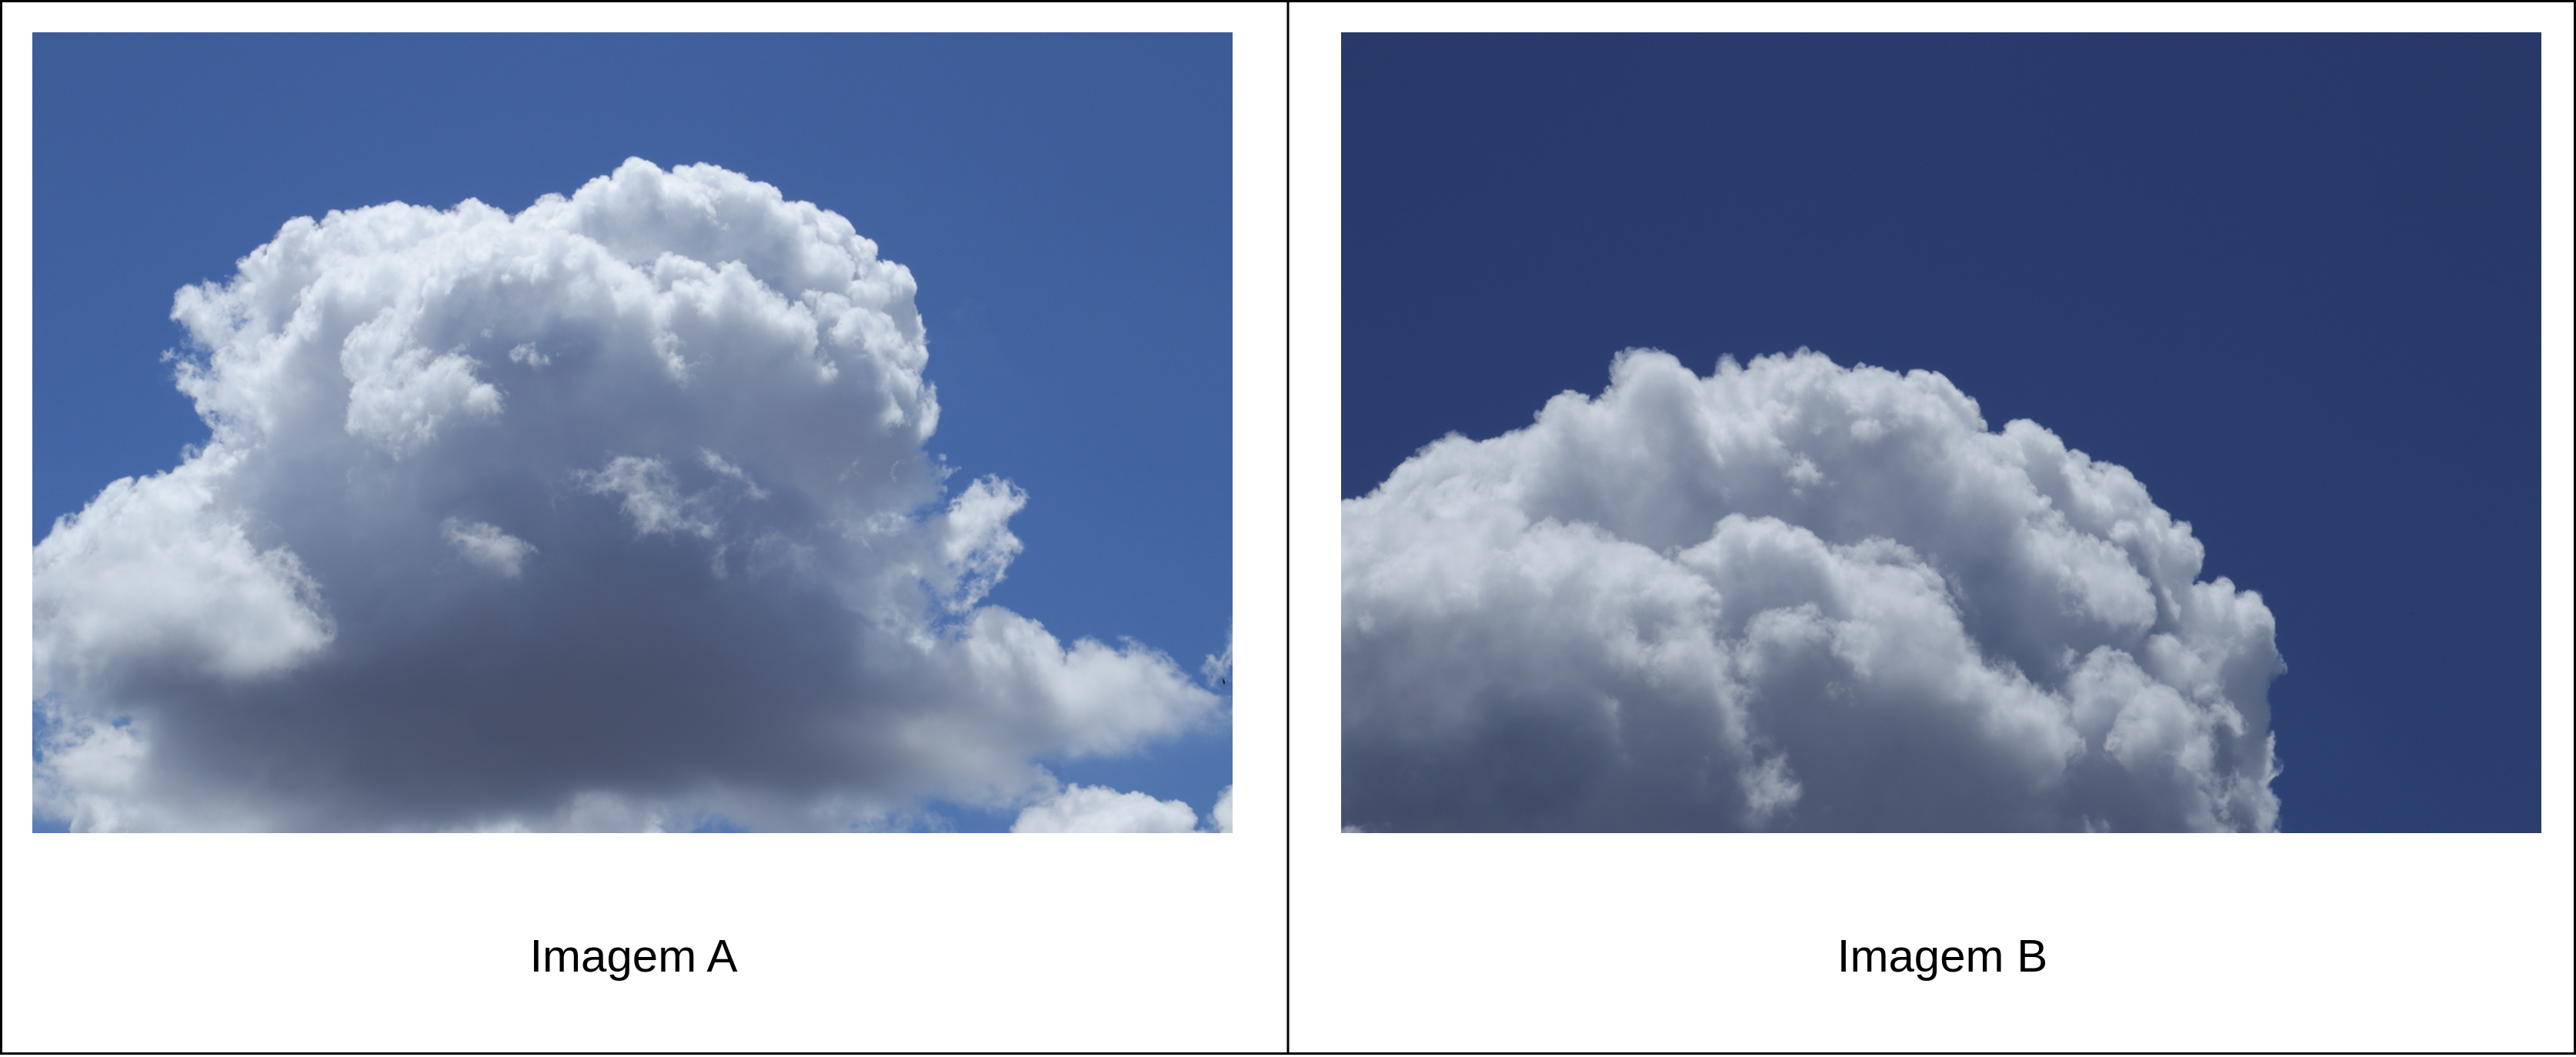
\includegraphics[width=14cm]{fig/similarity/image_a_and_image_b.png}
    \legend{Fonte: Autor (imagens e montagem).}
    \label{fig:fig32}
\end{figure}

Ao se executar o programa nas imagens da figura \ref{fig:fig32}, o resultado demonstrado na tabela \ref{tab:image_similarity_test} é obtido.

\begin{table}[H]
    \centering
    \caption{Tabela de resultados da execução do programa.}
    \begin{tabular}{|l|l|} \hline
        \textbf{Algoritmo} & \textbf{Resultado}      \\ \hline
        MSE                & 4259,146835763889       \\ \hline
        RMSE               & 65,26213937470858       \\ \hline
        PSNR               & 11,837577480628294      \\ \hline
        ERGAS              & 18054,91259300722       \\ \hline
    \end{tabular}
    \vspace{0.3cm}
    \legend{Fonte: Autor.}
    \label{tab:image_similarity_test}
\end{table}

Fazendo uma breve interpretação dos resultados, podemos concluir que a similaridade entre as imagens, como é de se esperar é baixa. A tabela \ref{tab:image_similarity_test_results_analysis}, descreve os resultados.

\begin{table}[H]
    \centering
    \caption{Tabela de descrição dos resultados da execução do programa.}
    \begin{tabular}{|l|l|l|} \hline
        \textbf{Algoritmo} & \textbf{Resultado} & \textbf{Análise}                        \\ \hline
        MSE                & 4259,146835763889  & Quanto mais próximo de 0, mais similar. \\ \hline
        RMSE               & 65,26213937470858  & Quanto mais próximo de 0, mais similar. \\ \hline
        PSNR               & 11,837577480628294 & Quanto maior o valor, mais similar.     \\ \hline
        ERGAS              & 18054,91259300722  & Quanto mais próximo de 0, mais similar. \\ \hline
    \end{tabular}
    \vspace{0.3cm}
    \legend{Fonte: Autor.}
    \label{tab:image_similarity_test_results_analysis}
\end{table}

Agora, apenas como meio de comparação, o programa será executado comparando agora, a imagem A com ela mesma. Os resultados estão na tabela \ref{tab:image_similarity_test_same_image}. 

\begin{table}[H]
    \centering
    \caption{Tabela de resultados da execução do programa com apenas a imagem A.}
    \begin{tabular}{|l|l|} \hline
        \textbf{Algoritmo} & \textbf{Resultado} \\ \hline
        MSE                & 0,0                \\ \hline
        RMSE               & 0,0                \\ \hline
        PSNR               & $\infty$           \\ \hline
        ERGAS              & 0,0                \\ \hline
    \end{tabular}
    \vspace{0.3cm}
    \legend{Fonte: Autor.}
    \label{tab:image_similarity_test_same_image}
\end{table}

\subsection{Coleta das imagens para avaliação dos resultados}

O treinamento das redes adversárias geradoras, produz algumas imagens com as quais o próprio programa de treinamento avalia a performance do modelo. No entanto, a quantidade de imagens produzidas durante o treinamento não é significativa para propriamente se avaliar como o modelo evoluiu após o treinamento.

Para coletar uma quantidade considerável de imagens, basta alimentar o modelo já treinado e armazenar a imagem resultante. No modelo utilizado, é necessário organizar as imagens desejadas em um diretório específico, obedecendo obviamente a estrutura requerida e preencher, com o caminho do diretório, o arquivo de configuração.


\subsubsection{Bases de dados utilizadas para a coleta de dados}

\begin{itemize}
    \item Base de dados médica \ref{sec:imagens_medicas}
    \item Base de dados astronômica \ref{sec:imagens_astronomicas}
\end{itemize}

\subsubsection{Programa para extração de estatísticas das imagens}
\label{sec:programa-extracao-estatisticas-imagem}

O processo de alimentar uma imagem em resolução reduzida à rede já treinada para em seguida formalmente compará-la, utilizando-se dos métodos de similaridade apresentados anteriormente (\ref{sec:qualidade-imagem}) à sua versão original é tedioso e mecânico: características comuns em tarefas automatizáveis.

Para tornar o processo mais eficiente, um programa codificado em \textit{Python} foi implementado. O programa, de forma superficial realiza as seguintes tarefas:

\begin{enumerate}
    \item De um arquivo de configuração, lê uma lista de bases de dados contendo as seguintes informações sobre cada:
    \begin{itemize}
        \item Nome
        \item Caminho do diretório contento os arquivos originais (imagens em alta resolução)
        \item Caminho do diretório contendo os arquivos extraídos da RAG (as mesmas imagens acima, com resoluções reduzidas e alimentadas à RAG)
        \item Extensão dos arquivos
    \end{itemize}
    \item Para cada uma das bases de dados, o programa:
    \begin{itemize}
        \item Lê as imagens do diretório com as imagens já passadas pela RAG
        \item Encontra a imagem equivalente no diretório contendo as imagens originais
        \item Como as imagens originais podem ter dimensões levemente diferentes das imagens que saem da RAG, o programa redimensiona a maior entre as duas imagens, para as dimensões da menor.
        \item Utilizando a biblioteca mencionada na seção \ref{sec:experimentos-similaridade-imagens}, produz um objeto contendo as estatísticas para todas as imagens contidas nos diretórios da configuração.
        \item Salva o objeto como um arquivo \textit{JSON}
    \end{itemize}
\end{enumerate}

\subsubsection{Análise dos resultados}

Uma ferramenta renomada no meio de análise e processamento de dados, é o \textit{Jupyter Notebook}. A ferramenta, consiste em um servidor, provedor de um interpretador interativo no navegador. Este interpretador, fornece de forma direta e eficaz um método para executar várias vezes seguidas, trechos de código, sem precisar de executar novamente o programa inteiro.

A ferramenta é perfeita para a análise dos dados produzidos na seção \ref{sec:programa-extracao-estatisticas-imagem}. Com os arquivos \textit{JSON} em mãos, um para a base de dados de ressonância magnética e outro para a base de dados astronômica, é possível extrair destes os dados e assim criar visualizações para análise dos resultados.




\chapter{Resultados}
\quot{``A vida é longa\\se você sabe usá-la``.\\Lúcio Sêneca}
\label{chapter:resultados}
Nesta parte, serão descritos os resultados obtidos, após todo o desenvolvimento elaborado anteriormente. Abaixo, gráficos e seus respectivos comentários serão detalhados. Os objetivos desta seção são visualizar e compreender como o ETE (Erro do treinamento específico) se compara com ETG (Erro do treinamento genérico). Os indicadores de desempenho, serão os métodos matemáticos para verificar similaridade entre imagens, descritos na seção \ref{sec:qualidade-imagem}. 

\section{Amostras das imagens resultantes}
\label{sec:amostra-img-resultante}

As figuras \ref{fig:img-results:fig1} e \ref{fig:img-results:fig2} são amostras aleatoriamente extraídas das bases de dados de ressonância magnética e astronômica, respectivamente. Em cada uma das figuras, a imagem \textbf{a} representa a imagem original assim como foi obtida da fonte. A imagem \textbf{b} representa a imagem \textbf{a}, após ser comprimida e passada pelo modelo treinado com o TG (Treinamento genérico). A imagem \textbf{c}, representa a imagem \textbf{a}, comprimida e alimentada ao modelo treinado pelo TE (Treinamento específico).

\begin{figure}[H]
    \centering
    \caption{Amostra aleatoriamente capturada das imagens de ressonância.}
    \begin{tabular}{c c c}
        \includegraphics[width=2.8cm]{fig/samples/mri/mri_original.png} & \includegraphics[width=2.8cm]{fig/samples/mri/mri_non_specific_training.png} & \includegraphics[width=2.8cm]{fig/samples/mri/mri_specific_training.png} \\
        (a) & (b) & (c)
    \end{tabular}
    \legend{Fonte: Autor}
    \label{fig:img-results:fig1}
\end{figure}


\begin{figure}[H]
    \centering
    \caption{Amostra aleatoriamente capturada das imagens de astronomia.}
    \begin{tabular}{c c c}
        \includegraphics[width=2.8cm]{fig/samples/astronomy/astronomy_original.png} & \includegraphics[width=2.8cm]{fig/samples/astronomy/astronomy_non_specific_training.png} & \includegraphics[width=2.8cm]{fig/samples/astronomy/astronomy_specific_training.png} \\
        (a) & (b) & (c)
    \end{tabular}
    \legend{Fonte: Autor}
    \label{fig:img-results:fig2}
\end{figure}

\section{Visualização dos resultados}
\label{sec:visualizacao-resultado}

Todas as imagens abaixo, possuem um gráfico superior, com os valores reais dos erros calculados, assim como uma regressão polinomial de primeiro grau e uma regressão polinomial de maior grau. Este gráfico está representado em escala logarítmica para os erros MSE e RMSE, devido à grande dispersão observada na visualização. Dessa forma, a imagem é mais compacta e concisa. 


A regressão de primeiro grau permite visualizar uma tendência geral dos dados e a regressão de maior grau aproximará ainda mais dos pontos distribuídos. As regressões fornecem uma melhor ideia de qual dos casos obteve um erro maior.

As imagens também possuem um histograma no gráfico inferior, representando a distribuição dos erros para ambos os cenários estudados, treinamento genérico e treinamento específico.

\subsection{Considerações gerais sobre os gráficos de resultados}
\label{sec:result:consideracoes-gerais}

Todas as imagens abaixo contém, no gráfico geral, os seguintes componentes:

\begin{itemize}
    \item Os pontos em azul, representando o valor do ETE.
    \item Os pontos em laranja, representando o valor do ETG.
    \item A estrela em vermelho, representando o valor mínimo do ETE.
    \item A estrela em azul, representando o valor mínimo do ETG.
    \item A estrela em amarelo, representando o valor máximo do ETE.
    \item A estrela em verde, representando o valor máximo do ETG.
    \item A curva em verde, representando o polinômio de primeiro grau, originado da regressão dos valores do ETE.
    \item A curva em vermelho escuro, representando o polinômio de primeiro grau, originado da regressão dos valores do ETG.
    \item A curva pontilhada em roxo, representando o polinômio de 40º grau, originado da regressão dos valores do ETE.
    \item A curva pontilhada em marrom, representando o polinômio de 40º grau, originado da regressão dos valores do ETG.
    \item Um histograma com a distribuição dos erros na parte inferior das imagens
\end{itemize}

\subsection{Estudo de resultados envolvendo a base de dados de ressonância magnética}
\label{sec:result:mri}
\subsubsection{Erro quadrático médio (MSE)}
\label{sec:result:mri:mse}

Começando com o erro quadrático médio, ao comparar a similaridade das imagens super resolvidas pela rede genericamente treinada com a similaridade das imagens super resolvidas pela rede treinada especificamente para lidar com imagens de ressonância magnética, são obtidos os resultados abaixo:

\begin{figure}[H]
    \centering
    \caption{Cálculo de erro MSE para base de dados de ressonância magnética.}
    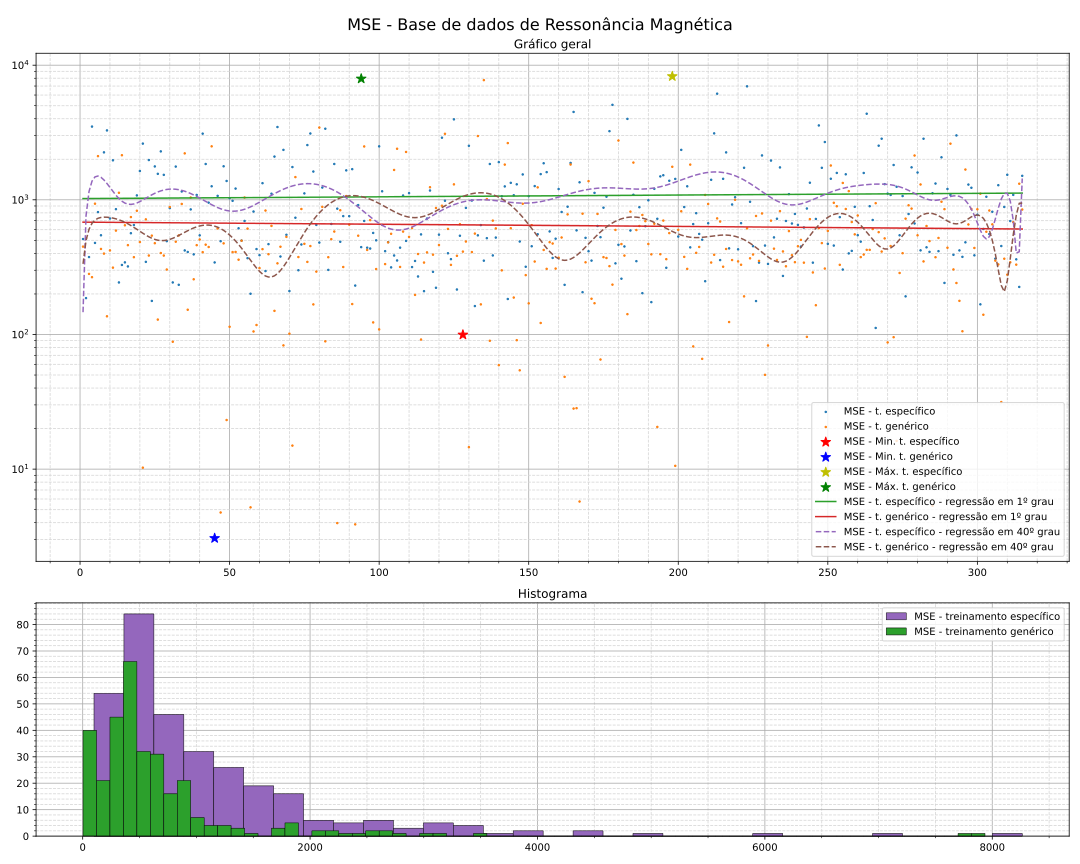
\includegraphics[width=10cm]{fig/resultados/mri/png/mse_mri_compound.png}
    \legend{Fonte: Autor}
    \label{fig:results:fig1}
\end{figure}

Os erros da figura \ref{fig:results:fig1} foram maiores nas imagens treinadas de forma específica. É notável que os polinômios relativos ao treinamento específico estão, em sua maior parte, acima dos polinômios do treinamento genérico. 

A mesma conclusão pode ser tirada, ao analisar a distribuição dos valores no histograma. A distribuição dos valores do ETE estão deslocadas mais à direita da distribuição do ETG. 


\subsubsection{Raiz do erro quadrático médio (RMSE)}
\label{sec:result:mri:rmse}


\begin{figure}[H]
    \centering
    \caption{Cálculo de erro RMSE para base de dados de ressonância magnética.}
    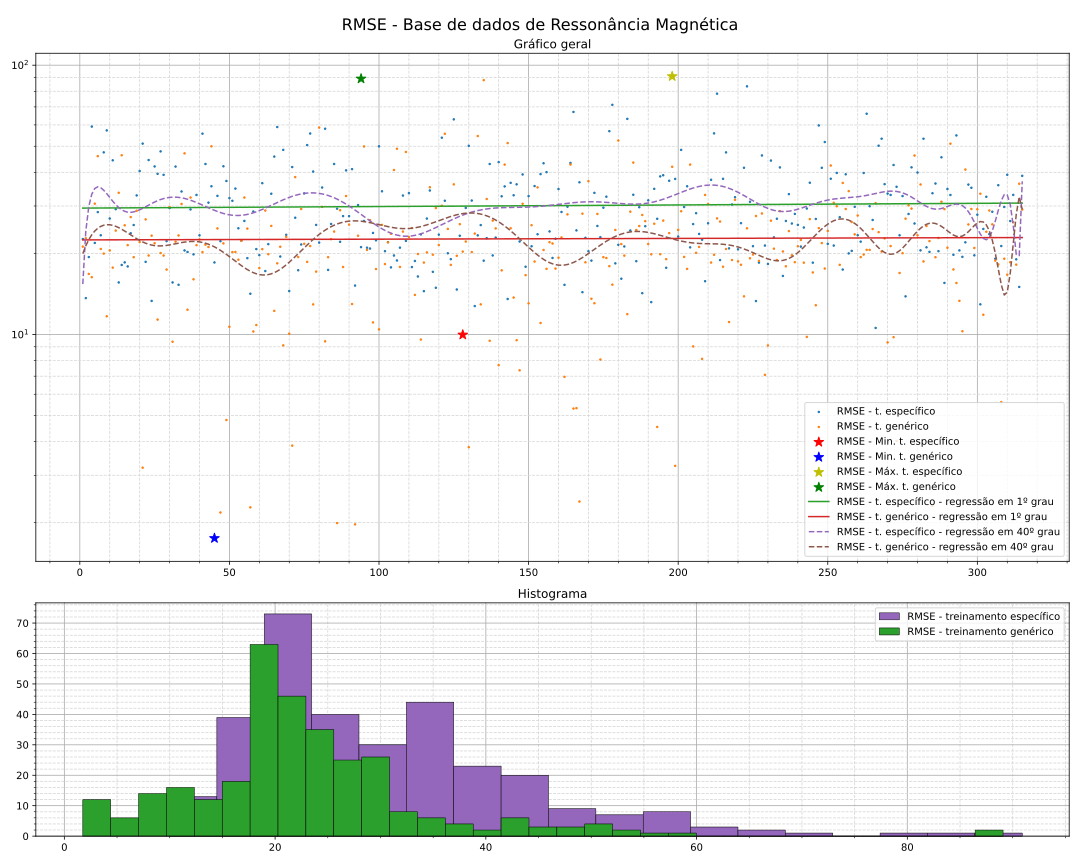
\includegraphics[width=10cm]{fig/resultados/mri/png/rmse_mri_compound.png}
    \legend{Fonte: Autor}
    \label{fig:results:fig2}
\end{figure}

O gráfico da figura \ref{fig:results:fig2} trás resultados muito similares aos da figura \ref{fig:results:fig1}, porém a variação do erro é menor. Enquanto no caso da figura \ref{fig:results:fig1} os valores se concentram entre 10 e 10000 para todas as amostras, para o erro RMSE, o intervalo é mais restrito: entre 0 e 100. Isso se deve à raiz quadrada, inexistente no cálculo do erro MSE.

Os resultados que podem ser extraídos do gráfico e histograma são praticamente idênticos aos extraídos da figura \ref{fig:results:fig1}. O treinamento específico da rede, produziu imagens com erros maiores que o treinamento genérico. 

\subsubsection{Relação sinal-ruído de pico (PSNR)}
\label{sec:result:mri:psnr}

\begin{figure}[H]
    \centering
    \caption{Cálculo de erro PSNR para base de dados de ressonância magnética.}
    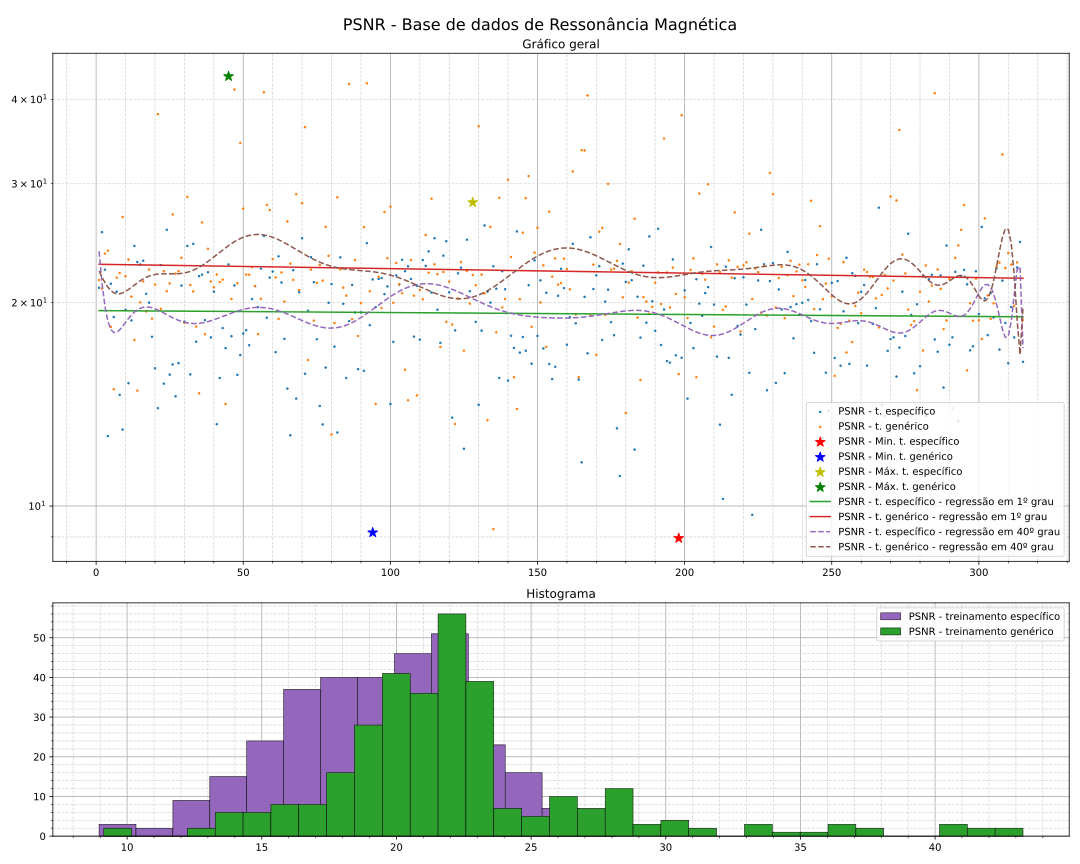
\includegraphics[width=10cm]{fig/resultados/mri/png/psnr_mri_compound.png}
    \legend{Fonte: Autor}
    \label{fig:results:fig3}
\end{figure}

Para esse erro em específico, a análise se inverte. Como descrito na seção \ref{sec:qualidade-imagem}, a similaridade entre as imagens é diretamente proporcional ao erro PSNR, enquanto nos casos anteriores a proporção era inversa.

Na figura \ref{fig:results:fig3}, mesmo utilizando uma escala logarítmica, observa-se bastante variação nas amostras. Seria difícil extrair significado destes dados sem as regressões polinomiais, dada tamanha dispersão. 

Com as regressões, nota-se que o treinamento específico produziu erros PSNR mais próximos de zero em relação ao treinamento genérico. O histograma confirma esta análise, demonstrando o deslocamento à esquerda das amostras do treinamento específico.

\subsubsection{Erro adimensional de síntese global relativa (ERGAS)}
\label{sec:result:mri:ergas}

\begin{figure}[H]
    \centering
    \caption{Cálculo de erro ERGAS para base de dados de ressonância magnética.}
    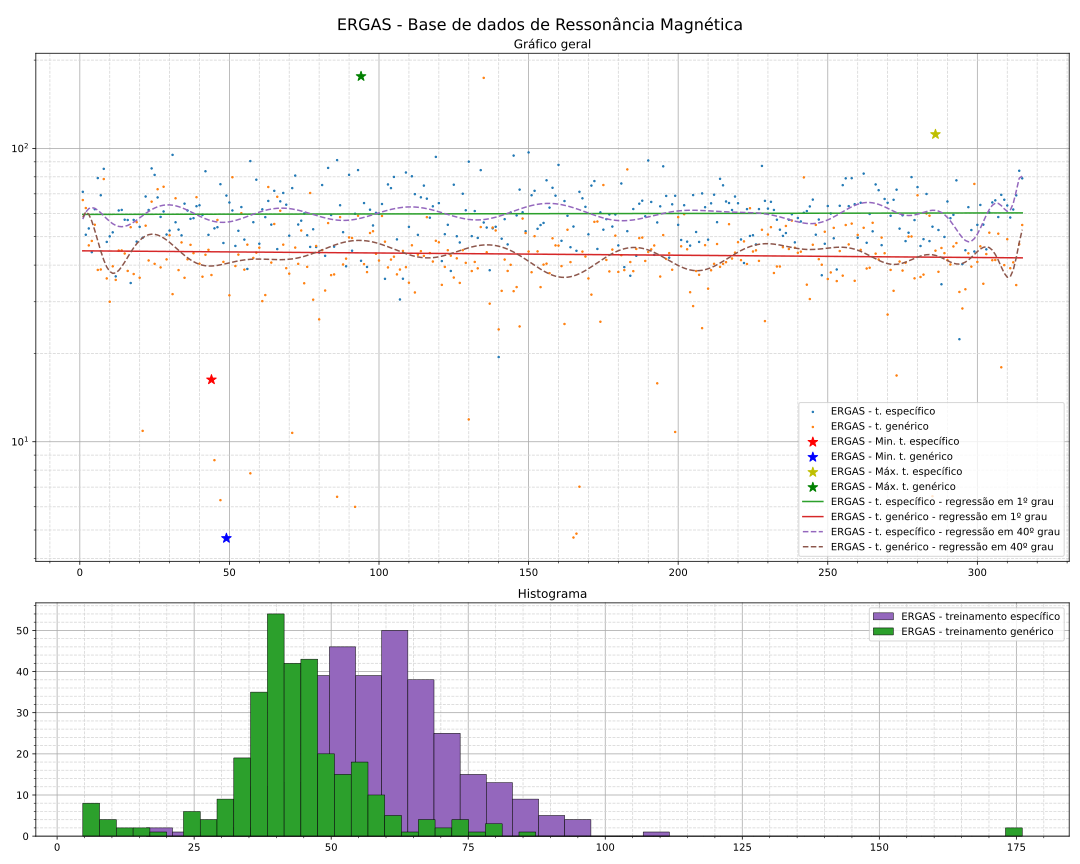
\includegraphics[width=10cm]{fig/resultados/mri/png/ergas_mri_compound.png}
    \legend{Fonte: Autor}
    \label{fig:results:fig4}
\end{figure}

O erro ERGAS da figura \ref{fig:results:fig4}, também produziu agrupamentos de amostras, mas dentro dos grupos, houve bastante variação entre os valores. Com as curvas de regressão no entanto, podemos claramente observar que o treinamento específico, novamente produziu erros maiores que o treinamento genérico. 

Assim como nas figuras \ref{fig:results:fig1} e \ref{fig:results:fig2}, a distribuição das amostras do ETE ficaram deslocadas à direita, evidenciando ainda mais o resultado antes descrito.

\subsection{Estudo de resultados envolvendo a base de dados de astronomia}
\label{sec:result:astronomy}

\subsubsection{Erro quadrático médio (MSE)}
\label{sec:result:astronomy:mse}

\begin{figure}[H]
    \centering
    \caption{Cálculo de erro MSE para base de dados astronômica.}
    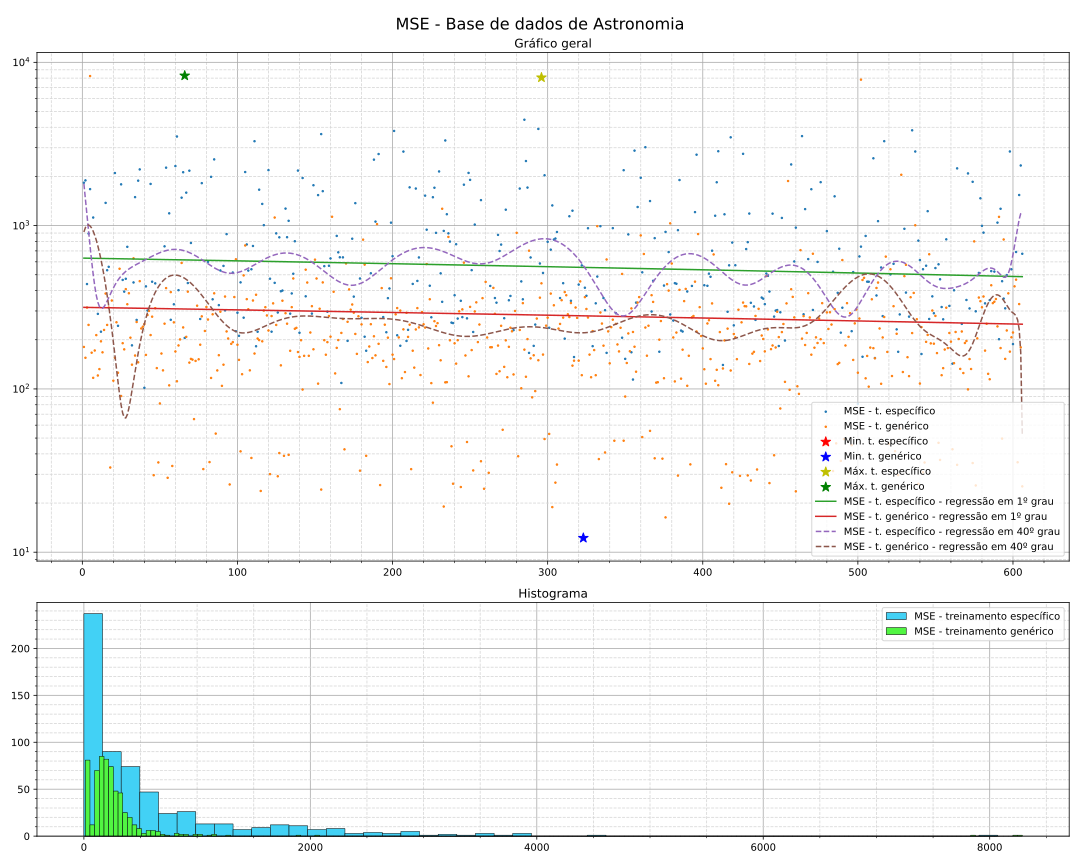
\includegraphics[width=10cm]{fig/resultados/astronomy/png/mse_astronomy_compound.png}
    \legend{Fonte: Autor}
    \label{fig:results:fig5}
\end{figure}

Na figura \ref{fig:results:fig5}, percebe-se com as regressões e o histograma que o ETE foi em sua maior parte, maior que o ETG. A distribuição do ETE se desloca à direita da distribuição do ETG.

\subsubsection{Raiz do erro quadrático médio (RMSE)}
\label{sec:result:astronomy:rmse}

\begin{figure}[H]
    \centering
    \caption{Cálculo de erro RMSE para base de dados astronômica.}
    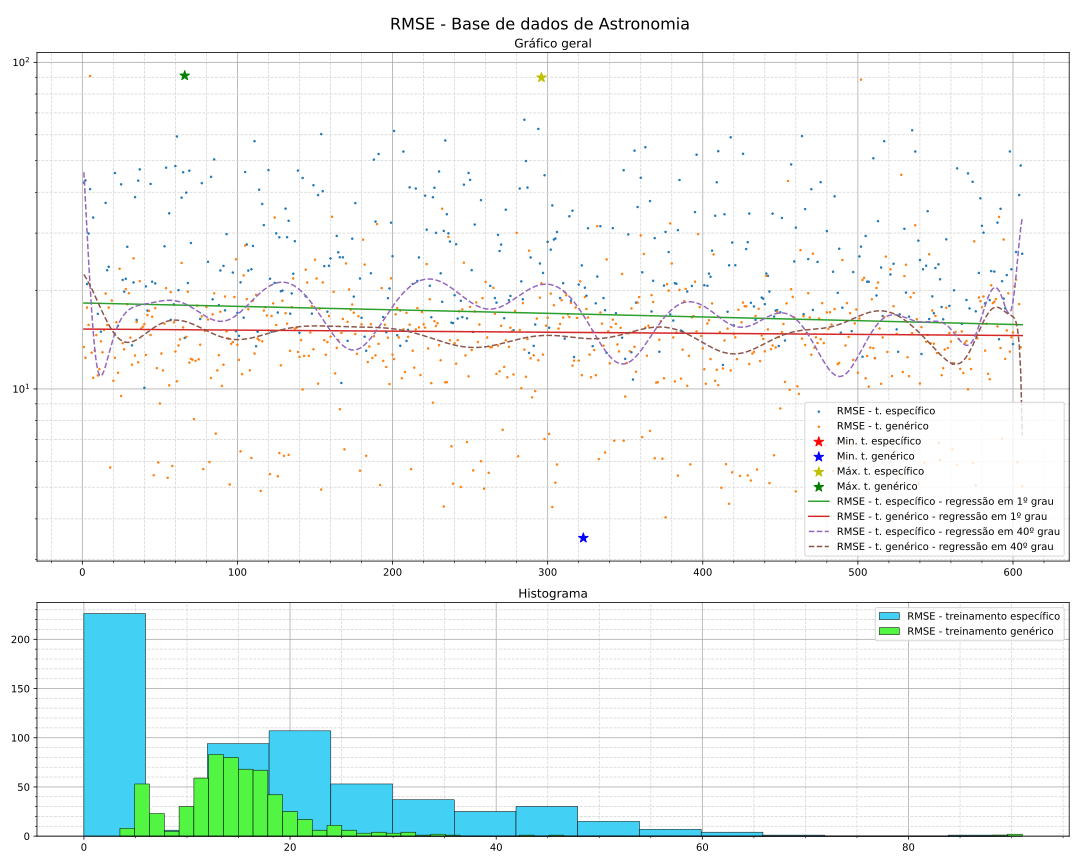
\includegraphics[width=10cm]{fig/resultados/astronomy/png/rmse_astronomy_compound.png}
    \legend{Fonte: Autor}
    \label{fig:results:fig6}
\end{figure}

A figura \ref{fig:results:fig6} traz resultados similares aos da figura \ref{fig:results:fig5}: o ETE é maior que o ETG. A principal diferença, como explicado anteriormente é o intervalo de distribuição reduzido de ambos os erros em relação à figura \ref{fig:results:fig5}.

\subsubsection{Relação sinal-ruído de pico (PSNR)}
\label{sec:result:astronomy:psnr}

\begin{figure}[H]
    \centering
    \caption{Cálculo de erro PSNR para base de dados astronômica.}
    \includegraphics[width=10cm]{fig/resultados/astronomy/png/psnr_astronomy_compound.png}
    \legend{Fonte: Autor}
    \label{fig:results:fig7}
\end{figure}

No gráfico da figura \ref{fig:results:fig7} é possível observar que os dois cenários formam agrupamentos. O ETE está deslocado para baixo do gráfico. O resultado extraído disso são condizentes com o que foi visto nos erros anteriores. O treinamento específico gerou erros PSNR mais próximos de zero e estão distribuídos mais à esquerda dos erros do treinamento genérico.

Note também que o distanciamento entre as regressões do ETE e as regressões do ETG foi maior, em relação ao erro PSNR calculado para a base de dados de ressonância magnética na seção \ref{sec:result:mri:psnr}. 

\subsubsection{Erro adimensional de síntese global relativa (ERGAS)}
\label{sec:result:astronomy:ergas}

\begin{figure}[H]
    \centering
    \caption{Cálculo de erro ERGAS para base de dados astronômica.}
    \includegraphics[width=10cm]{fig/resultados/astronomy/png/ergas_astronomy_compound.png}
    \legend{Fonte: Autor}
    \label{fig:results:fig8}
\end{figure}

Outra vez, na figura \ref{fig:results:fig8} o ETE é maior que o ETG e assim como no erro ERGAS da seção \ref{sec:result:mri:ergas}, a dispersão dificultaria a análise sem as regressões. Apesar disso, o resultado se mantém. O treinamento específico produziu imagens menos similares às originais.

\section{Considerações gerais sobre o resultado}
\label{sec:result:consideracoes-gerais}

No geral, o TE produziu resultados inferiores ao TG e isso foi fortemente evidenciado em cada um dos gráficos descritos anteriormente. Constante e consistentemente o ETG produziu erros menores que o ETE, excluindo naturalmente o PSNR em que a análise se inverte, e em consequência, o maior valor é o mais atraente, do ponto de vista de similaridade. Com os ajustes necessários, o ETE sempre apontou na direção de menor similaridade com as imagens originais e isso é notável até mesmo de forma subjetiva e visual, como demonstrado nas imagens \ref{fig:img-results:fig1} e \ref{fig:img-results:fig2} na seção \ref{sec:amostra-img-resultante}.


\chapter{Conclusão}
\quot{``Nem homem nem nação podem\\existir sem uma ideia sublime``.\\Fiódor Dostoiévski}
\label{chapter:conclusao}
Com os resultados descritos de forma técnica, uma conclusão sob estes é possibilitada. A proposta do trabalho, de verificar se treinar redes adversarias generativas especificamente para um determinado cenário produziria melhores resultados do que uma RAG treinada de forma genérica, foi fortemente desafiada pelos resultados, no quesito viabilidade. O trabalho documenta uma estratégia pouco otimizada de se realizar super resolução de imagens, especialmente se comparado ao estado da arte. No ponto de vista científico no entanto, este texto pode vir a conduzir futuros leitores para fora de um caminho pouco frutífero e que não trará resultados positivos. 

No que tangem os objetivos, sejam estes específicos ou geral, pode-se avaliar que o trabalho realizou a proposta apresentada. Alguns destes objetivos tiveram seus cumprimentos delongados devido a obstáculos impostos por diversos fatores técnicos. Outros, no entanto, foram cumpridos de maneira menos tortuosa. Este é o caso da definição das bases de imagens para treinamento dos modelos. Por mais que determinado esforço de pesquisa tenha sido necessário até que alternativas viáveis e cabíveis fossem encontradas e eventualmente as imagens nestas contidas fossem processadas para que se encaixassem nos requisitos impostos pelo modelo, todo esse processo foi antecipado nas fases de concepção deste trabalho.

Os objetivos específicos de definir o modelo a ser utilizado e de integração dos componentes de \textit{software} impuseram altos e baixos no fluxo de desenvolvimento. A definição do modelo envolveu muitas tentativas e erros, e vários candidatos em potencial foram descartados seja porque não funcionaram, ou porque se desempenharam de maneira pobre durante os testes preliminares, falhando seguidamente ou tomando muito tempo para falhar. Em um dos casos, o modelo treinou por horas durante a noite e falhou em algum momento da madrugada. Este objetivo anda de mãos atadas com o objetivo de integração, já que para que se defina um modelo que atenda ao escopo proposto, uma integração harmoniosa é indispensável. Como descrito detalhadamente na seção \ref{sec:environment-version-compatability}, um leque de compatibilidade teve de ser encontrado entre as variadas partes que compuseram o modelo utilizado e também os modelos descartados. Encontrar essa faixa de compatibilidade possui desafios próprios. Nem todo \textit{software} utilizado possui uma documentação clara e explícita sobre as bibliotecas que foram utilizadas em sua composição. Em consequência, mais uma vez, a tentativa e erro foi empregada de maneira exaustiva até que uma configuração funcional fosse estabelecida.

Na fase final do trabalho, o último objetivo que se refere à utilização de métodos de avaliação de similaridade de imagens para avaliação de custo-benefício se realizou. O processo em si envolveu bastante automação já que quantidades grandes de imagens estavam sendo testadas. Este objetivo é o último requisito para que se possa avaliar o objetivo geral do trabalho.  

Os resultados obtidos pelo TE (treinamento específico) foram constantemente inferiores aos resultados obtidos pelo TG (Treinamento genérico). Em todos os métodos de avaliação utilizados (MSE, RMSE, PSNR e ERGAS) o TE produziu um desempenho pior. Algumas hipóteses podem ser levantadas sobre as razões pelas quais tais resultados foram obtidos.

A primeira das hipóteses é a limitação de recursos computacionais para o treinamento específico. Para executar o treinamento na máquina disponível, apenas duas imagens eram colocadas em memória por iteração, ou seja, um \textit{batch size} de dois. No contrário, problemas de memória impediriam o treinamento. Para fins de comparação, o modelo treinado por \citeonline{wang_esrgan_2018}, utilizou um \textit{batch size} de 16 e o modelo de \citeonline{wang_real-esrgan_2021}, uma evolução do anterior, utiliza um \textit{batch size} de 48. 

Além desta limitação de memória, há também a limitação de processamento e, conectada a isso, as restrições de tempo. Redes neurais complexas como as que compõem a ESRGAN são, geralmente, treinadas em servidores de alto desempenho, contendo múltiplos chips gráficos com dezenas de milhares de núcleo. Os treinamentos realizados para este trabalho, foram feitas em uma máquina pessoal, ordens de grandeza menos potente que as máquinas utilizadas pela indústria. Enquanto treinamentos profissionais acontecem por dias, o dispositivo utilizado neste trabalho não estava disponível vinte e quatro horas por dia para o treinamento. Tudo isso acarretou na redução de mais um parâmetro de configuração: o número total de épocas.

Para ambas as bases de dados, o treinamento específico foi feito por 100 épocas com 1000 iterações cada, um número baixo em comparação à treinamentos mais profissionais. Apesar disso, o modelo pré-treinado, obrigatório para especializar as redes, pode ter ajudado o desempenho do TE não ter sido ainda mais inferior ao desempenho do TG. TG que por sua vez, foi feito por terceiros em um ambiente com recursos muito mais abundantes. Apesar de não ser conhecido o número de épocas exato utilizado no modelo treinado genericamente, é possível ter uma ideia aproximada deste valor. O artigo de \citeonline{wang_esrgan_2018} menciona treinamentos de 50000, 100000, 200000 e 300000 iterações. Um segundo artigo feito em cima de uma melhoria ao modelo ESRGAN \cite{wang_real-esrgan_2021} detalha treinamentos de 400000 e 1000000 de iterações. Valores totalmente impraticáveis para os recursos disponíveis para a execução deste trabalho. Um treinamento com esta duração envolveria um comprometimento temporal muito grande. Estes valores se traduziriam em semanas, quiçá meses de uso intenso e ``ininterrupto'' do dispositivo utilizado para o treinamento, algo que foge do escopo do presente trabalho. A palavra ``ininterrupto'' foi escrita entre aspas por um motivo. O treinamento de fato, não pode ser interrompido, porém, existem formas de configurar o projeto para salvar pontos de checagem do modelo. Isso abre as portas para um trabalho futuro: explorar treinamentos longos, porém pausados e analisar os resultados.

Ambos modelos treinados nos artigos citados anteriormente, contaram com recursos computacionais de alto nível para o treinamento das redes. Tais dispositivos reduzem consideravelmente o tempo de treinamento, como mencionado na seção \ref{sec:environment-prep-training}. 

Outra hipótese diz respeito à disparidade entre os erros da base de ressonância magnética e de astronomia. Comparando as seções \ref{sec:result:mri} e \ref{sec:result:astronomy}, especialmente os erros PSNR (seções \ref{sec:result:mri:psnr} e \ref{sec:result:astronomy:psnr}) nota-se que o TE sob a base astronômica, apesar de ter sido realizado no mesmo dispositivo, com os mesmos parâmetros, produziu resultados piores que o TE da base de ressonância magnética. Existem duas diferenças críticas entre as duas bases de dados. Primeiro, a base de dados astronômica possui imagens coloridas. Segundo, como visto na seção \ref{sec:desenvolvimento:general-considerations-post-processed-images}, as imagens de ressonância magnética são menores em disco que as imagens astronômicas. Ambas as diferenças impõem obstáculos para o TE das imagens astronômicas. 

Imagens coloridas, são mais complexas estruturalmente que imagens monocromáticas (vide diagrama da figura \ref{fig:monochrome_vs_color}). Considerando os mesmos recursos e parâmetros utilizados para um treinamento, é seguro dizer que o treinamento realizado sobre imagens coloridas produzirá resultados inferiores. Quando se trata de imagens coloridas, as dimensões das estruturas internas de dados aumentam em algumas vezes. Uma imagem de largura L, altura A em tons de cinza possui uma estrutura bidimensional L por A, cada posição contendo a intensidade do respectivo pixel. A mesma imagem, agora com três canais de cores (vermelho, verde e azul), possui a mesma estrutura, porém repetida três vezes, uma para cada canal. Logo, há mais informação para ser analisada e mais informação para as redes se especializarem. Um trabalho futuro pode ser extraído destas disparidades: refazer os treinamentos com bases de imagens mais uniformes.

O desempenho do TE, mesmo que inferior ao TG, poderia ter sido significativamente pior. Na seção de desenvolvimento \ref{sec:preping-project-for-training}, foi descrito que para treinar as redes, um modelo pré-treinado seria necessário, para que o treinamento em si não precisasse aprender do zero. Dessa forma, a redes puderam se especializar em cima de algo já treinado, mesmo que minimamente. 

O maior desafio deste trabalho não foi a revisão bibliográfica, não foi compreender conceitos complexos de aprendizado de máquina e também não foi o esforço para encontrar e processar bases de imagens acessíveis de forma pública e gratuita. Apesar de todas estas fases citadas terem requerido um esforço significativo, o maior obstáculo, e em consequência, onde o maior aprendizado foi concretizado, foram as integrações de softwares de terceiros um com o outro, podendo-se utilizar apenas da documentação provida pelos desenvolvedores. Documentação que embora essencial, não foi suficiente para garantir o funcionamento de ponta a ponta. Bastante tentativa e erro foi empregada neste processo de integração. 

O trabalho desenvolvido, aponta que dado recursos reduzidos ou disputados por outras tarefas, utilizar um modelo de super resolução baseado em redes geradoras adversárias do tipo ESRGAN treinado de forma genérica, trará resultados mais satisfatórios.




\chapter{Propostas de trabalhos futuros}
\quot{``Feliz é aquele que transfere o\\que sabe e aprende o que ensina.``\\Cora Coralina}
\label{chapter:trabalhos_futuros}
\index{Trabalhos futuros}
\label{sec:trabalhos-futuros}

Durante todo o processo de pesquisa e execução deste trabalho, várias outras possíveis aplicações de super-resolução foram detectadas. Seja como uma inteira nova utilidade ou como uma variação deste trabalho. A ideia aqui é documentar algumas possíveis ideias extraídas do trabalho atual.

\section{Uso de RAGs com imagens geográficas}
\label{sec:trabalhos-futuros:imagens-geograficas}

\subsection{Super resolução de imagens de satélites}
\label{sec:trabalhos-futuros:imagens-geograficas:imagens-satelites}

Existe na internet um acervo bem completo e extenso de imagens aéreas e de satélites, algumas destas bem antigas. Ferramentas como \textit{Google Earth} permitem viajar no passado, para visualizar como diversas regiões eram anos atrás. Estas imagens, apesar de impressionantes, têm baixa resolução. Geralmente, quanto mais antigas as imagens, menor a resolução. O trabalho proposto é de utilizar a super resolução com GAN para restaurar tais imagens e talvez até produzir um mapa mais refinado. 

\subsection{RAGs e drones de baixo custo para mapeamento geográfico}
\label{sec:trabalhos-futuros:imagens-geograficas:mapeamento-geografico-drone}

Fazer um mapeamento geográfico de uma região com detalhes suficientes para extrair detalhes de estruturas como prédios, casas etc. utilizando de técnicas de fotogrametria pode ser um processo caro. Equipamentos que possuem os recursos necessários e boa resolução têm preços consideráveis. Com uma forma confiável de fazer super resolução de imagens, equipamentos inferiores, e em consequência mais baratos, podem ser utilizados para fazer o escaneamento aéreo, e no pós processamento, a ideia é super resolver as imagens produzidas para prosseguir então com o mapeamento. 

\section{Uso de RAGs para compressão e descompressão de imagens e vídeos}
\label{sec:trabalhos-futuros:compressao-descompressao}

Como dito no final da seção \ref{justificativa}, o uso de RAGs para super resolução de imagens pode trazer uma forma de descompressão de imagens como subproduto. Todo mundo atualmente possui uma câmera poderosa em seus bolsos e armazenar grandes quantidades de fotos e vídeos, produzidos em grande escala diariamente, é um problema comum enfrentado pelo usuário médio. Caso seja possível comprimir estas imagens e vídeos -- que não passam de uma sequência de imagens -- sob demanda, descomprimi-los com fidelidade suficiente para que não seja um problema para o usuário, assume-se então que um método eficiente de descompressão de imagens foi desenvolvido. 

\section{Uso de RAGs para microscopia}
\label{sec:trabalhos-futuros:microscopia}

\subsection{Super resolução de imagens microscópicas}
\label{sec:trabalhos-futuros:microscopia:imagens-existentes}

Seguindo a mesma linha deste trabalho, como trabalho futuro a sugestão seria de usar bases de dados existentes para aprimorar a qualidade das imagens de microscopia disponíveis na internet. Aumentar a quantidade de detalhes em uma imagem de microscópio pode ser de grande ajuda para o público alvo deste tipo de conteúdo. 

\subsection{RAGs e microscópios caseiros de baixo custo}
\label{sec:trabalhos-futuros:microscopia:baixo-custo}

Existem diversas formas de se fabricar um microscópio com tecnologias acessíveis como \textit{WebCams} de entrada. Apesar da facilidade para se produzir tal equipamento, como é de se esperar, a qualidade das imagens geradas não possui grande qualidade. A proposta, seria de utilizar tal ferramenta em conjunto com uma RAG para super resolver as imagens -- talvez em tempo real, mostrando diretamente em um display a imagem já super resolvida. Este trabalho produziria uma forma barata e eficaz de se observar e analisar objetos microscópicos. 

\section{Uso de RAGs em monitoramento}
\label{sec:trabalhos-futuros:monitoramento}

\subsection{RAGs e câmeras de segurança}
\label{sec:trabalhos-futuros:monitoramento:camera-seguranca}

\subsubsection{RAGs para redução de armazenamento (compressão e descompressão)}
\label{sec:trabalhos-futuros:monitoramento:camera-seguranca:compressao-descompressao}

Um dos problemas existentes com sistemas de segurança é o armazenamento dos vídeos capturados. Até quando manter um vídeo armazenado? O máximo possível é a melhor alternativa. Contudo, o tempo máximo possível é obviamente limitado pelo armazenamento disponível. Os gravadores de vídeo digital (conhecidos como DVR) utilizados em sistemas de segurança costumam utilizar a gravação contínua até encher os discos rígidos. Uma vez completamente cheios, o armazenamento mais antigo vai sendo sobrescrito à medida que vídeo subsequente é gravado. A proposta seria comprimir estes vídeos, e posteriormente descomprimi-los com boa qualidade e fidelidade ao material original, para aumentar significativamente este período máximo de retenção de imagens. 

\subsubsection{RAGs para captura de detalhes refinados}
\label{sec:trabalhos-futuros:monitoramento:camera-seguranca:extracao-detalhes}

Identificar objetos em imagens de câmeras de segurança não é uma tarefa simples. A resolução baixa muitas vezes não permite extrair informações importantes como identidade de pessoas ou identificação de veículos. Com uma forma eficiente de super resolver estas imagens, talvez seja possível mudar a forma de analisar vídeos e imagens de sistemas de segurança. 

\subsection{Monitoramento de trânsito}
\label{sec:trabalhos-futuros:monitoramento:transito}

Assim como no caso acima (seção \ref{sec:trabalhos-futuros:monitoramento:camera-seguranca:extracao-detalhes}), o objetivo nesta proposta é aprimorar o detalhe de imagens produzidas por câmeras de baixa resolução. Obter identificação de veículos pode ser positivamente afetado por uma ferramenta de super resolução de imagens de câmeras de trânsito. 

\section{Super resolução para entretenimento}
\label{sec:trabalhos-futuros:entretenimento}

\subsection{RAGs para jogos}
\label{sec:trabalhos-futuros:entretenimento:jogos}

O objetivo seria a utilização de RAGs para remasterizar jogos antigos originalmente produzidos para dispositivos de baixa resolução. 

\subsection{RAGs para filmes e séries}
\label{sec:trabalhos-futuros:entretenimento:filmes-series}

O intuito desta proposta é a utilização de RAGs para, assim como o caso acima (\ref{sec:trabalhos-futuros:entretenimento:jogos}), aumentar a resolução e definição da imagem. Existem diversas ferramentas que já fazem este tipo de tarefa. Este trabalho seria um estudo de caso. Neste tópico, um adendo poderia ser construir um aplicativo ou ferramenta para facilitar a execução destas super resoluções. Desta forma, o público não técnico poderia tirar proveito dos resultados. 

\section{Super resolução de áudio}
\label{sec:trabalhos-futuros:audio}

Áudio digital possui uma frequência de gravação e uma taxa de amostragem limitadas pela capacidade dos equipamentos e software utilizados na gravação e mixagem. A proposta deste trabalho seria aumentar esta frequência sem reduzir significativamente a fidelidade do áudio. Existem formas tradicionais de ampliar esta frequência (ou resolução) como interpolação, mas estes mecanismos não são inteligentes o suficiente para detectar padrões que outrora podem ser identificados por um modelo de aprendizado de máquina como RAGs. 

Uma RAG, composta por redes capazes de extrair contexto espacial dos dados de entrada, talvez seja capaz de interpolar estatisticamente amostras de áudio entre amostras existentes, criando assim um áudio digital mais encorpado e próximo à sua contraparte analógica. 

\section{Portabilidade do trabalho atual}
\label{sec:trabalhos-futuros:portabilidade}

O presente trabalho necessita de um desktop ou servidor rodando o modelo para executá-lo. Para utilizar a versão móvel, ainda assim é necessário um \textit{backend} processando os dados e os enviando para o dispositivo móvel. Algumas bibliotecas de inteligência artificial como o \textit{Tensorflow} possuem versões dedicadas para executar em dispositivos móveis. Alguns dispositivos possuem até mesmo hardware dedicado para este tipo de processamento, como a \textit{Neural Engine} utilizada pela \textit{Apple} e alguns de seus produtos. A proposta deste trabalho futuro seria portar o modelo atual ou um modelo similar para dispositivos móveis de forma a eliminar a necessidade de uma infraestrutura inteira para o funcionamento da ferramenta. Esta proposta pode ainda transformar o trabalho em um produto.

\section{Estudo sobre a viabilidade de treinamentos pausados}
\label{sec:trabalhos-futuros:treinamento-pausado}

Como mencionado na seção \ref{chapter:conclusao}, existe a possibilidade de se realizar um treinamento pausado em ciclos. A proposta para este trabalho futuro seria experimentar sobre esta técnica, coletando dados para elaborar sobre a viabilidade de se treinar um modelo por esse método. Planejamento e agendamento das atividades será essencial para realizar um treinamento longo. Diferentemente do trabalho atual, uma atividade dessas requer pontualidade para executar os ciclos de treinamento: enquanto neste trabalho, todos treinamentos do modelo foram feitos em uma única execução, na proposta, o treinamento seria feito por um número de épocas por execução, até atingir-se um resultado satisfatório.


\bookmarksetup{startatroot}

\postextual

\bibliography{references}

\printindex

\end{document}
